\documentclass{scrreprt}

\usepackage{amsmath}
\usepackage{mathtools}
\usepackage{amssymb}
\usepackage[hidelinks]{hyperref}
\usepackage{algorithm}
\usepackage[noend]{algpseudocode}
% \usepackage{algorithmicx}
\usepackage{amsthm}
\usepackage{graphicx}
\usepackage{animate}
\usepackage{booktabs}
\usepackage{tabulary}
\usepackage{rotating}

\makeatletter
\newcounter{algorithmbis}
\setcounter{algorithmbis}{0}
\renewcommand{\thealgorithmbis}{\arabic{algorithmbis}}
\def\algorithmbis{\@ifnextchar[{\@algorithmbisa}{\@algorithmbisb}}
\def\@algorithmbisa[#1]{%
  \refstepcounter{algorithmbis}
  \trivlist
  \leftmargin\z@
  \itemindent\z@
  \labelsep\z@
  \item[\parbox{\textwidth}{%
    \hrule
    \hrule
    \noindent\strut\textbf{Algorithm \thealgorithmbis} #1
    \hrule
  }]\hfil\vskip0em%
}
\def\@algorithmbisb{\@algorithmbisa[]}
\def\endalgorithmbis{\hfil\vskip-1em\hrule\endtrivlist}
\makeatother

\DeclareMathOperator*{\argmin}{arg\,min}
\DeclareMathOperator*{\argmax}{arg\,max}
\DeclareMathOperator{\Bin}{Bin}
\DeclareMathOperator{\Ber}{Ber}
\DeclareMathOperator{\Beta}{Beta}
\DeclareMathOperator{\BetaBin}{BetaBin}
\DeclareMathOperator{\Cat}{Cat}
\DeclareMathOperator{\Dir}{Dir}
\DeclareMathOperator{\DirMult}{DirMult}
\DeclareMathOperator{\Mult}{Mult}
\DeclareMathOperator{\Poi}{Poi}
\DeclareMathOperator{\Gammadist}{Gamma}
\DeclareMathOperator{\NB}{NB}
\DeclareMathOperator{\Unif}{Unif}
\DeclareMathOperator{\Pareto}{Pareto}
\DeclareMathOperator{\Gauss}{\mathcal N}
\DeclareMathOperator{\E}{\mathrm{E}}
\DeclareMathOperator{\var}{\mathrm{var}}
\DeclareMathOperator{\cov}{\mathrm{cov}}
\DeclareMathOperator{\grad}{\mathrm{grad}}
\newcommand*\mean[1]{\bar{#1}}
\DeclareMathOperator{\diag}{diag}
\DeclareMathOperator{\KL}{KL}
\DeclareMathOperator{\Tr}{Tr}
\DeclareMathOperator{\I}{\mathbb I}

\renewcommand{\vec}[1]{\boldsymbol{\mathbf{#1}}}
\newtheorem{definition}{Definition}[section]
\newtheorem{theorem}{Theorem}[section]
\newtheorem{proposition}{Proposition}[section]
\newtheorem{claim}{Claim}[section]

\bibliographystyle{plain}

\allowdisplaybreaks
\title{Personal notes -- Bayesian machine learning}
\author{Tuan Anh Le}

\begin{document}
\maketitle
\tableofcontents

\chapter{Notation}
\begin{tabular}{ll}
    $\left\{a_n\right\}$                & Same as $\left\{a_n\right\}_{n = 1}^N$ and $\left\{a_1, \dotsc, a_N\right\}$ -- denotes a set of sequence \\
    $\vec x \in R^D$                    & $D$-dimensional real-valued vector \\
    $\sum_k f(\cdot)$                   & Shorthand for $\sum_{k = 1}^K f(\cdot)$ (for an arbitrary index letter) \\
    $\prod_k f(\cdot)$                  & Shorthand for $\prod_{k = 1}^K f(\cdot)$ (for an arbitrary index letter) \\
    $\diag(x_1, \dotsc, x_N)$           & Diagonal matrix formed from the elements $x_1, \dotsc, x_N$. \\
    $I(\cdot)$							& Indicator function, equal to 1 if the argument is true, 0 otherwise.
\end{tabular}
\chapter{Basics}
\section{Probability distributions}
Summarised in Table~\ref{table:prob-dist}

\begin{sidewaystable}[htp!]
\label{table:prob-dist}
\begin{tabulary}{0.75\textheight}{cccccc}
\toprule
Distribution & Parameters & Support & PDF/PMF & Mean & Variance \\
\midrule
Bernoulli ($\Ber$)

&

$\theta \in [0, 1]$

& 

$x \in \{0, 1\}$

&

\(\displaystyle
	\begin{cases}
		\theta 		& \text{if } x = 1 \\
		1 - \theta	& \text{if } x = 0
	\end{cases}
\)

&

$\theta$

&

$\theta (1 - \theta)$ \\
Beta ($\Beta$)

&

$\alpha, \beta > 0$

&

$x \in [0, 1]$

&

\(\displaystyle
	\frac{\Gamma(\alpha + \beta)}{\Gamma(\alpha)\Gamma(\beta)} x^{\alpha - 1} (1 - x)^{\beta - 1}
\)

&

$\frac{\alpha}{\alpha + \beta}$

&

$\frac{\alpha\beta}{(\alpha + \beta)^2(\alpha + \beta + 1)}$ \\
Binomial ($\Bin$)

&

$N \in \mathbb N, \theta \in [0, 1]$

& 

$x \in \{0, \dotsc, N\}$

&

\(\displaystyle
	p(x) = \binom{N}{x} \theta^x (1 - \theta)^{N - x}
\)

& 

$N\theta$

&

$N\theta(1 - \theta)$ \\
Beta-Binomial ($\BetaBin$)

&

$N \in \mathbb N, \alpha, \beta > 0$

&

$x \in \{0, \dotsc, N\}$

&

\(\displaystyle
	\binom{N}{x} \frac{B(x + \alpha, N - x + \beta)}{B(\alpha, \beta)}
\)

& 

$\frac{N\alpha}{\alpha + \beta}$

&

$\frac{N\alpha\beta(\alpha + \beta + N)}{(\alpha + \beta)^2(\alpha + \beta + 1)}$ \\
Poisson ($\Poi$)

&

$\lambda > 0$

& 

$x \in \mathbb \{0, 1, 2, \dotsc\}$

&

\(\displaystyle
	\frac{\lambda^x}{x!} \exp(-\lambda)
\)

& 

$\lambda$

&

$\lambda$ \\
Gamma ($\Gammadist$)

&

$\alpha, \beta > 0$

& 

$x > 0$

&

\(\displaystyle
	p(x) = \frac{\beta^{\alpha}}{\Gamma(\alpha)} x^{\alpha - 1} \exp(-\beta x)
\)

& 

$\frac{\alpha}{\beta}$

&

$\frac{\alpha}{\beta^2}$ \\
Negative-Binomial ($\NB$)

&

$r > 0, p \in (0, 1)$

& 

$x \in \{0, 1, 2, \dotsc\}$

&

\(\displaystyle
	p(x) = \frac{\Gamma(x + r)}{x!\,\Gamma(r)} (1 - p)^r p^x
\)

& 

$\frac{pr}{1 - p}$

&

$\frac{pr}{(1 - p)^2}$ \\
\bottomrule
\end{tabulary}
\caption{Summary of common probability distributions}\footnote{where $B(\alpha, \beta)$ is the normalisation constant for a Beta distribution, $\Beta(\alpha, \beta)$, which is $\int_x x^{\alpha - 1} (1 - x)^{\beta - 1} \,\mathrm d x$ or $\frac{\Gamma(\alpha)\Gamma(\beta)}{\Gamma(\alpha + \beta)}$.}
\end{sidewaystable}
\section{Stats}
\subsection{Kolmogorov-Smirnov test}
\subsubsection{Kolmogorov-Smirnov statistic}
Null hypothesis, often denoted by $H_0$ is a general statement or a default position saying there is no relationship between two measured phenomena. 

The Kolmogorov (KS) test quantifies a distance between
\begin{itemize}
	\item The empirical distribution function (or the empirical cdf) and the cdf of the reference function ($H_0 = $ sample is drawn from the reference distribution), or
	\item The empirical cdfs of two samples ($H_0 = $ samples are drawn from the same distribution).
\end{itemize}

The empirical cdf $F_N$ for $N$ iid observations $\{x_n\}$ is
\begin{equation}
	F_N(x) \triangleq \frac{1}{N} \sum_n I(x_n \leq x)
\end{equation}
basically $F_N(x) = \frac{1}{N} \text{number of samples less than or equal to } x$.

The KS statistic for a given cdf $F(x)$ is
\begin{equation}
	D_N(x) \triangleq \sup_x \left|F_N(x) - F(x)\right|
\end{equation}
By Glivenko-Cantelli theorem, if $\{x_n\} \sim F$, then $D_N \to 0$ almost surely when $N \to \infty$.
\subsection{Kullback-Leibler divergence}
A.k.a. \emph{KL divergence}, or \emph{relative enropy}. KL divergence between the distributions $p(\vec x)$ and $q(\vec x)$ for $\vec x \in \mathcal X$, denoted $\KL(p \parallel q)$ or $\KL(p, q)$, is a measure of similarity between $p$ and $q$ and is given by
\begin{align}
    \KL(p \parallel q)  &= -\int_{\mathcal X} p(\vec x) \ln q(\vec x) \,\mathrm d\vec x - \left(-\int_{\mathcal X} p(\vec x) \ln p(\vec x) \,\mathrm d\vec x\right) \nonumber\\
                        &= -\int_{\mathcal X} p(\vec x) \ln \frac{q(\vec x)}{p(\vec x)} \,\mathrm d\vec x
\end{align}

Note that $\KL(p \parallel q) \not\equiv \KL(q \parallel p)$.

\begin{claim}
    $\KL(p \parallel q) \geq 0$ with equality if and only if $p(\vec x) = q(\vec x)$.
\end{claim}

\begin{proof}
    asdf
\end{proof}
\section{Gaussian distribution}
The density of $\vec x \sim \Gauss\left(\vec \mu, \vec \Sigma\right), \vec x \in \mathbb R^D$ is
\begin{align}
    p(\vec x)   &= \frac{1}{\sqrt{|2\pi\vec \Sigma|}} \exp{\left[-\frac{1}{2}(\vec x - \vec \mu)^T \vec \Sigma^{-1} (\vec x - \vec \mu)\right]} \\
                &= (2\pi)^{-D / 2} |\vec \Sigma|^{-1 / 2} \exp{\left[-\frac{1}{2}(\vec x - \vec \mu)^T \vec \Sigma^{-1} (\vec x - \vec \mu)\right]}
\end{align}
\subsection{Linear Gaussian model}
\label{ssec:prob-gaussian-lingauss}
Given the marginal and conditional distributions to be
\begin{align}
    p(\vec x)               &= \Gauss(\vec x; \vec \mu, \vec \Lambda^{-1}) \label{eqn:prob-gaussian-lingauss1} \\
    p(\vec y \mid \vec x)   &= \Gauss(\vec y; \vec A \vec x + \vec b, \vec L^{-1}) \label{eqn:prob-gaussian-lingauss2}
\end{align}
the marginal distribution of $\vec y$ and the conditional distribution of $\vec x$ given $\vec y$ are given by
\begin{align}
    p(\vec y)               &= \Gauss\left(\vec y; \vec A \vec \mu + \vec b, \vec L^{-1} + \vec A \vec \Lambda^{-1} \vec A^T\right) \label{eqn:prob-gaussian-lingauss3}\\
    p(\vec x \mid \vec y)   &= \Gauss\left(\vec x; \vec \Sigma\left\{\vec A^T \vec L(\vec y - \vec b) + \vec \Lambda \vec \mu\right\}, \vec \Sigma\right) \label{eqn:prob-gaussian-lingauss4}
\end{align}
where
\begin{equation}
    \vec \Sigma = \left(\vec \Lambda + \vec A^T \vec L \vec A \right)^{-1} \label{eqn:prob-gaussian-lingauss5}
\end{equation}

\paragraph{Why it works}
\chapter{Bayesian parameter estimation}
Given a set of data $\mathcal D = \{\vec x_n \}$, we impose a probability distribution $f$ with parameters $\vec \theta$, which we call the model parameters, on each data point, $\vec x_n \sim f(\vec \theta), n = 1, \dotsc, N$, so that the likelihood becomes $p(\mathcal D \mid \vec \theta) = \prod_n f(\vec x_n \mid \vec \theta)$. We also impose a distribution $g$ on $\vec \theta$ with parameters $\vec \alpha$ which we call the hyperparameters. We call this distribution, the prior distribution over $\vec \theta$. Bayesian parameter estimation evaluates the posterior distribution, $p(\vec \theta \mid \mathcal D)$, and the posterior predictive distribution, $p(\tilde{\vec x} \mid \mathcal D)$, where $\tilde{\vec x}$ is a new data point we want to predict.

When the prior $g(\vec \theta \mid \vec \alpha)$ is a conjugate prior for a given likelihood distribution $f(\cdot \mid \vec \theta)$, the posterior has the same distribution as $g$, just with different parameters. We call these updated hyperparameters, and denote them by adding a dash, $\vec \alpha'$. In other words, the posterior becomes $g(\vec \theta \mid \vec \alpha')$. Table~\ref{table:par-est} summarises the quantities of interest for several conjugate pairs, followed by the derivations.

\begin{sidewaystable}[htp!]
\label{table:par-est}
\begin{tabulary}{1\textheight}{CCCCCC}
\toprule
Likelihood 	& Model parameters				& Prior 	& Hyperparameters  				& Posterior Hyperparameters 												& Posterior predictive \\ \midrule
Bernoulli	& $\theta$						& Beta 		& $\alpha, \beta$  				& $\alpha + \sum_n \I(x_n = 1), \beta + \sum_n \I(x_n = 0)$	& $\Ber\left(\tilde x \mid \frac{\alpha'}{\alpha' + \beta'}\right)$ \\
Binomial	& $\theta$						& Beta 		& $\alpha, \beta$  				& $\alpha + \sum_n x_n, \beta + \sum_n (T_n - x_n)$							& $\BetaBin(\tilde x \mid \alpha', \beta')$ \\
Poisson		& $\lambda$						& Gamma 	& $\alpha, \beta$  				& $\alpha + \sum_n x_n, \beta + N$											& $\NB\left(\tilde x \mid \alpha', \frac{1}{1 + \beta'}\right)$ \\
Categorical	& $\vec \theta \in \mathbb R^K$	& Dirichlet	& $\vec \alpha \in \mathbb R^K$	& $\vec \alpha + (n_1, \dotsc, n_K)^T$										& $\Ber\left(\tilde x \mid \frac{{\alpha'}_{\tilde x}}{\sum_k \alpha'_k}\right)$ \\
Multinomial	& $\vec \theta \in \mathbb R^K$	& Dirichlet	& $\vec \alpha \in \mathbb R^K$	& $\vec \alpha + \sum_n \vec x_n$											& $\DirMult(\tilde{\vec x} \mid \alpha', \tilde T)$ \\
\bottomrule
\end{tabulary}
\caption{Summary of Bayesian parameter estimation for conjugate pairs} 
\end{sidewaystable}

\section{Beta-Bernoulli model}
\subsection{Summary}
\paragraph{The model}
    \begin{align}
        X_i         &\sim \Ber(\theta), \text{for } i \in \{1, \dotsc, N\} \\
        \mathcal D  &= \{x_1, \dotsc, x_N\} \\
        N_1         &= \sum_{i = 1}^N \mathbb I (x_i = 1) \\
        N_0         &= \sum_{i = 1}^N \mathbb I (x_i = 0)
    \end{align}

\paragraph{Likelihood}
    \begin{equation}
        p(\mathcal D | \theta) = \theta^{N_1} (1 - \theta)^{N_0}
    \end{equation}

\paragraph{Prior}
    \begin{equation}
        p(\theta)   = \Beta(\theta | a, b)
    \end{equation}

\paragraph{Posterior}
    \begin{equation}
        p(\theta | \mathcal D) = \Beta(\theta | a' = N_1 + a, b' = N_0 + b)
    \end{equation}

\paragraph{Posterior predictive}
    \begin{equation}
        p(\tilde x = 1 | \mathcal D) = \frac{a'}{a' + b'}
    \end{equation}

\paragraph{Evidence}

\subsection{Derivations}

\section{Beta-Binomial model}
$\mathcal D = \{x_n : x_n \sim \Bin(T_n, \theta)\}$ for some fixed total counts $\{T_n\}$, $\theta \sim \Beta(\alpha, \beta)$.

\paragraph{Likelihood.}
    \begin{align*}
        p(\mathcal D \mid \theta)   &= \prod_n \Bin(x_n \mid T_n, \theta) \\
                                    &\propto \prod_n \theta^{x_n} (1 - \theta)^{T_n - x_n} \\
                                    &= \theta^{\sum_n x_n} (1 - \theta)^{\sum_n T_n - x_n} \\
                                    &= \theta^{x} (1 - \theta)^{T - x} \\
                                    &\propto \Bin(x \mid T, \theta)
    \end{align*}
where $x = \sum_n x_n$ and $T = \sum_n T_n$.

\paragraph{Posterior.}
    \begin{align*}
        p(\theta \mid \mathcal D)   &\propto p(\mathcal D \mid \theta) p(\theta) \\
                                    &= \Bin(x \mid T, \theta) \Beta(\theta \mid \alpha, \beta) \\
                                    &\propto \theta^{x} (1 - \theta)^{T - x} \theta^{\alpha - 1} (1 - \theta)^{\beta - 1} \\
                                    &= \theta^{\alpha + x - 1} (1 - \theta)^{\beta + T - x - 1} \\
                                    &\propto \Beta(\theta \mid \alpha + x, \beta + T - x) \\
                                    &= \Beta\left(\theta \mid \alpha + \sum_n x_n, \beta + \sum_n (T_n - x_n)\right)
    \end{align*}

\paragraph{Posterior predictive.} (New data point $\tilde x$ for some fixed total count $\tilde T$).
    \begin{align*}
        p(\tilde x \mid \mathcal D, \tilde T)   &= \int_{\theta} p(\tilde x, \theta \mid \mathcal D, \tilde T) \,\mathrm d\theta \\
                                                &= \int_{\theta} p(\tilde x \mid \theta, \mathcal D, \tilde T) p(\theta \mid \mathcal D, \tilde T) \,\mathrm d\theta \\
                                                &= \int_{\theta} p(\tilde x \mid \theta, \tilde T) p(\theta \mid \mathcal D) \,\mathrm d\theta \\
                                                &= \int_{\theta} \Bin(\tilde x \mid \tilde T, \theta) \Beta(\theta \mid \alpha', \beta') \,\mathrm d\theta \\
                                                &= \int_{\theta} \left[\binom{\tilde T}{\tilde x} \theta^{\tilde x} (1 - \theta)^{\tilde T - \tilde x}\right] \left[\frac{1}{B(\alpha', \beta')} \theta^{\alpha' - 1} (1 - \theta)^{\beta' - 1}\right] \,\mathrm d\theta \\
                                                &= \binom{\tilde T}{\tilde x} \frac{1}{B(\alpha', \beta')} \int_{\theta} \theta^{\tilde x + \alpha' - 1} (1 - \theta)^{\tilde T - \tilde x + \beta' - 1} \,\mathrm d\theta \\
                                                &= \binom{\tilde T}{\tilde x} \frac{B(\alpha' + \tilde x, \beta' + \tilde T - \tilde x)}{B(\alpha', \beta')} \\
                                                &= \BetaBin(\tilde x \mid \tilde T, \alpha', \beta')
    \end{align*}
where $B(\alpha, \beta)$ is the normalisation constant for a Beta distribution, $\Beta(\alpha, \beta)$, which is $\int_x x^{\alpha - 1} (1 - x)^{\beta - 1} \,\mathrm dx$ or $\frac{\Gamma(\alpha)\Gamma(\beta)}{\Gamma(\alpha + \beta)}$.
\section{Poisson-Gamma model}
$\mathcal D = \{x_n : x_n \sim \Poi(\lambda)$, $\lambda \sim \Gammadist(\alpha, \beta)$.

\paragraph{Likelihood.}
    \begin{align*}
        p(\mathcal D \mid \lambda) &= \prod_n \Poi(x_n \mid \lambda)
    \end{align*}

\paragraph{Posterior.}
    \begin{align*}
        p(\lambda \mid \mathcal D)  &\propto p(\mathcal D \mid \lambda) p(\lambda) \\
                                    &= \left(\prod_n \Poi(x_n \mid \lambda) \right) \Gammadist(\lambda \mid \alpha, \beta) \\
                                    &\propto \left[\prod_n \frac{\lambda^{x_n}}{x_n!} \exp(-\lambda)\right] \left[\lambda^{\alpha - 1} \exp(-\lambda\beta)\right] \\
                                    &\propto \lambda^{\alpha + \sum_n x_n - 1} \exp(-\lambda(\beta + N)) \\
                                    &\propto \Gammadist\left(\lambda \mid \alpha + \sum_n x_n, \beta + N\right)
    \end{align*}

\paragraph{Posterior predictive.}
    \begin{align*}
        p(\tilde x \mid \mathcal D) &= \int_{\lambda} p(\tilde x, \lambda \mid \mathcal D) \,\mathrm d\lambda \\
                                    &= \int_{\lambda} p(\tilde x \mid \lambda, \mathcal D) p(\lambda \mid \mathcal D) \,\mathrm d\lambda \\
                                    &= \int_{\lambda} p(\tilde x \mid \lambda) p(\lambda \mid \mathcal D) \,\mathrm d\lambda \\
                                    &= \int_{\lambda} \Poi(\tilde x \mid \lambda) \Gammadist(\lambda \mid \alpha', \beta') \,\mathrm d\lambda \\
                                    &= \int_{\lambda} \frac{\lambda^{\tilde x}}{\tilde x!} \exp(-\lambda) \frac{1}{G(\alpha', \beta')} \lambda^{\alpha' - 1} \exp(-\beta' \lambda) \,\mathrm d\lambda \\
                                    &= \frac{1}{\tilde x! G(\alpha', \beta')} \int_{\lambda} \lambda^{x + \alpha' - 1} \exp(-\lambda (\beta' + 1)) \,\mathrm d\lambda \\
                                    &= \frac{G(\alpha' + x, \beta + 1)}{\tilde x! G(\alpha', \beta')} \\
                                    &= \frac{\Gamma(\alpha' + \tilde x)}{\tilde x! \Gamma(\alpha')} \cdot \frac{\beta'^{\alpha'}}{(\beta' + 1)^{\alpha' + \tilde x}} \\
                                    &= \frac{\Gamma(\alpha' + \tilde x)}{\tilde x! \Gamma(\alpha')} \left(1 - \frac{1}{1 + \beta'}\right)^{\alpha'} \left(\frac{1}{1 + \beta'}\right)^{\tilde x} \\
                                    &= \NB\left(\tilde x \mid \alpha', \frac{1}{1 + \beta'}\right)
    \end{align*}
where $G(\alpha, \beta)$ is the normalisation constant for a Gamma distribution, $\Gammadist(\alpha, \beta)$, which is $\int_x x^{\alpha - 1} \exp(-\beta x) \,\mathrm dx$ or $\frac{\Gamma(\alpha)}{\beta^\alpha}$.
\section{Dirichlet-Categorical model}
$\mathcal D = \{x_n : x_n \sim \Cat(\vec\theta), \vec\theta \in \mathbb R^K\}$, $\vec\theta \sim \Dir(\vec\alpha), \alpha \in \mathbb R^K$.

\paragraph{Likelihood.}
    \begin{align*}
        p(\mathcal D \mid \vec \theta) &= \prod_k \theta_k^{n_k}
    \end{align*}
    where $n_k = \sum_n \I(x_n = k)$.

\paragraph{Posterior.}
    \begin{align*}
        p(\vec \theta \mid \mathcal D)  &\propto p(\mathcal D \mid \vec \theta) p(\vec \theta) \\
                                        &= \prod_k \theta_k^{n_k} \Dir(\vec \theta \mid \vec \alpha) \\
                                        &\propto \prod_k \theta_k^{n_k} \prod_k \theta_k^{\alpha_k - 1} \\
                                        &= \prod_k \theta_k^{\alpha_k + n_k - 1} \\
                                        &\propto \Dir\left(\vec \theta \mid \vec \alpha + (n_1, \dotsc, n_K)^T\right)
    \end{align*}

\paragraph{Posterior predictive.}
    \begin{align*}
        p(\tilde x \mid \mathcal D)     &= \int_{\vec \theta} p(\tilde x, \vec \theta \mid \mathcal D) \,\mathrm d\vec\theta \\
                                        &= \int_{\vec \theta} p(\tilde x \mid \vec \theta, \mathcal D) p(\vec \theta \mid \mathcal D) \,\mathrm d\vec\theta \\
                                        &= \int_{\vec \theta} p(\tilde x \mid \vec \theta) p(\vec \theta \mid \mathcal D) \,\mathrm d\vec\theta \\
                                        &= \int_{\vec \theta} \Cat(\tilde x \mid \vec \theta) \Dir(\vec \theta \mid \vec \alpha') \\
                                        &= \int_{\vec \theta} \theta_{\tilde x} \Dir(\vec \theta \mid \vec \alpha') \,\mathrm d\vec\theta \\
                                        &= \E_{\vec \theta \sim \Dir(\vec \alpha')}[\theta_{\tilde x}] \\
                                        &= \frac{\alpha'_{\tilde x}}{\sum_k \alpha'_k}
    \end{align*}

\paragraph{Evidence.}
    \begin{align}
        p(\mathcal D)   &= \frac{p(\mathcal D \given \vec\theta)p(\vec\theta)}{p(\vec \theta \given \mathcal D)} \nonumber\\
                        &= \frac{\left(\prod_k \theta_k^{n_k}\right)\left(\Dir(\vec\theta \given \alpha\right))}{\Dir\left(\vec \theta \given \alpha + (n_1, \dotsc, n_K)^T\right)} \nonumber\\
                        &= \frac
                            {
                                \left(\prod_k \theta_k^{n_k}\right)
                                \frac
                                    {\Gamma\left(\sum_k \alpha_k\right)}
                                    {\prod_k \Gamma(\alpha_k)}
                                \left(\prod_k \theta_k^{\alpha_k - 1}\right)
                            }
                            {
                                \frac
                                    {\Gamma\left(N + \sum_k \alpha_k\right)}
                                    {\prod_k \Gamma(\alpha_k + n_k)}
                                \left(\prod_k \theta_k^{\alpha_k + n_k - 1}\right)
                            } \nonumber\\
                        &= \frac
                            {
                                \Gamma\left(\sum_k \alpha_k\right)
                                \prod_k \Gamma(\alpha_k + n_k)
                            }
                            {
                                \Gamma\left(N + \sum_k \alpha_k\right)
                                \prod_k \Gamma(\alpha_k)
                            } \label{eqn:bayes/par-est/dir-cat/evidence}
    \end{align}
\section{Dirichlet-multinomial model}
\subsection{Summary}
\paragraph{The model}
    \begin{align}
        \vec N      &\sim \Mult(N, \vec\theta) \in \mathbb R^K \\
        \mathcal D  &= \{\vec n = \text{vector of counts of successes}\} \\
        N           &= \sum_{i = 1}^K n_i \\
        \tilde{\mathcal D} &= \{\tilde{\vec n} = \text{vector of counts of successes in a new batch of data}\} \\
        \tilde N          &= \sum_{i = 1}^K \tilde n_i
    \end{align}

\paragraph{Likelihood}
    \begin{equation}
        p(\mathcal D | \theta) = \Mult(\vec n; N, \vec\theta)
    \end{equation}

\paragraph{Prior}
    \begin{equation}
        p(\theta)   = \Dir(\vec\theta; \vec\alpha)
    \end{equation}

\paragraph{Posterior}
    \begin{equation}
        p(\theta | \mathcal D) = \Dir(\vec\theta; \vec\alpha' = \vec\alpha + (n_1, \dotsc, n_K)^T)
    \end{equation}

\paragraph{Posterior predictive}
    \begin{align}
        p(\tilde{\mathcal D} | \mathcal D) &= \frac{\Gamma(\alpha_0 + N)}{\Gamma(\alpha_0 + N + \tilde N)} \prod_{k = 1}^K \frac{\Gamma(\alpha_k + n_k + \tilde n_k)}{\Gamma(\alpha_k + n_k)} \\
        \text{where } \alpha_0 &= \sum_{k = 1}^K \alpha_k
    \end{align}

\paragraph{Evidence}
    \begin{equation}
        p(\mathcal D | \vec\alpha) = \frac{\Gamma(\alpha_0)}{\Gamma(\alpha_0 + N)} \prod_{k = 1}^K \frac{\Gamma(\alpha_k + n_k)}{\Gamma(\alpha_k)}
    \end{equation}

\subsection{Derivations}
\input{par-est/unif-pareto}
\chapter{Generative models}
\chapter{Sampling algorithms}
\section{Introduction}
    Let $p$ be a probability distribution with pdf $p(\vec x)$, which we assume can be evaluated within a multiplicative factor (i.e. we can only evaluate $p^\ast(\vec x) = Z_p p(\vec x)$, where $Z_p = \int p^\ast(\vec x)\,\mathrm d\vec x$). We want to achieve the following:
    \begin{description}
        \item[Problem 1] Generate samples $\{\vec x^{(1)}, \dotsc, \vec x^{(R)}\}$ (shorthand notation $\{\vec x^{(r)}\}$) from the probability distribution $p$.
        \item[Problem 2] Estimate the expectation of an arbitrary function $f$ given that $\vec x \sim p$, $\E [f]$. 
    \end{description}

\section{Rejection sampling}

Assume we can sample from a proposal distribution $q$ with a pdf $q(\vec x)$, which can be evaluated within a multiplicative factor (i.e. we can only evaluate $q^\ast(\vec x) = Z_q q(\vec x)$). Also assume we know the value of a constant $c$ such that
\begin{align}
    c q^\ast(\vec x) > p^\ast(\vec x) & \text{ for all } \vec x
\end{align}

The procedure that generates a sample $\vec x \sim p$ is described in Algorithm~\ref{alg:rejection} below.
\begin{algorithm}
\caption{Rejection sampling}\label{alg:rejection}
    \begin{algorithmic}[1]
        \State Generate $\vec x \sim q$.
        \State Generate $u \sim \Unif(0, c q^\ast(\vec x))$.
        \State If $u > p^\ast(\vec x)$ it is rejected, otherwise it is accepted.
    \end{algorithmic}
\end{algorithm}


\subsection{Why it works?}
    Assume $\vec x \in \mathbb R^D$. Define sets $\mathcal X$ and $\mathcal X'$ to be
    \begin{align}
        \mathcal X &= \left\{\vec \alpha \in \mathbb R^{d + 1}: \alpha_{1:d} \in \mathbb R^d, \alpha_{d + 1} \in [0, c q^\ast(\vec \alpha)]\right\} \\
        \mathcal X' &= \left\{\vec \alpha \in \mathbb R^{d + 1}: \alpha_{1:d} \in \mathbb R^d, \alpha_{d + 1} \in [0, p^\ast(\vec \alpha)]\right\}
    \end{align}
    Note that $\mathcal X' \subseteq \mathcal X$.

    By definition, $\mathcal X$ is the support of $(\vec x, u)$. The probability of $(\vec x, u)$ can be expressed as
    \begin{align}
        \Pr(\vec x, u)  &= \Pr(\vec x) \Pr(u) \\
                        &= q(\vec x) \frac{1}{c q^\ast(\vec x)} \\
                        &= q(\vec x) \frac{1}{c Z_q q(\vec x)} \\
                        &= \frac{1}{c Z_q}
    \end{align}
    which is constant w.r.t. $(\vec x, u)$, i.e.
    \begin{equation}
        (\vec x, u) \sim \Unif(\mathcal X)
    \end{equation}

    Let $(\vec x', u')$ be the value of $(\vec x, u)$ that gets accepted. By definition, $\mathcal X'$ is the support of $(\vec x', u')$:
    \begin{equation}
        (\vec x', u') =
            \begin{cases}
                (\vec x, u)     & \text{if } (\vec x, u) \in \mathcal X' \\
                \text{nothing}  & \text{otherwise.}
            \end{cases}
    \end{equation}
    The probability of $(\vec x', u')$ can be expressed as
    \begin{equation}
        \Pr(\vec x', u') =
            \begin{cases}
                \Pr(\vec x, u)  & \text{if } (\vec x, u) \in \mathcal X' \\
                0               & \text{otherwise.}
            \end{cases}
    \end{equation}
    which means
    \begin{equation}
        (\vec x', u') \sim \Unif(\mathcal X')
    \end{equation}

    Working backwards
    \begin{align}
        \Pr(\vec x')    &= \frac{\Pr(\vec x', u')}{\Pr(u')} \\
                        &\propto \frac{1}{1 / p^\ast(\vec x')} \\
                        &\propto p^\ast(\vec x')
    \end{align}
    Hence the accepted $\vec x$, $\vec x'$ is $\sim p$.
\section{Importance sampling}

Assume we can sample from a proposal distribution $q$ with a pdf $q(\vec x)$, which can be evaluated within a multiplicative factor (i.e. we can only evaluate $q^\ast(\vec x) = Z_q q(\vec x)$). To solve problem 2, we follow Algorithm~\ref{alg:importance} below.
\begin{algorithm}
\caption{Importance sampling}\label{alg:importance}
    \begin{algorithmic}[1]
        \State Generate samples from $q$, $\{\vec x^{(r)}\}$.
        \State Calculate importance weights $w_r = \frac{p^\ast(\vec x^{(r)})}{q^\ast(\vec x^{(r)})}$.
        \State $\hat{\vec y} = \frac{\sum_r w_r f(\vec x^{(r)})}{\sum_r w_r}$ is the estimator of $\E[f]$.
    \end{algorithmic}
\end{algorithm}

\subsection{Convergence of estimator as $R$ increases}
    We want to prove that if $q(\vec x)$ is non-zero for all $\vec x$ where $p(\vec x)$ is non-zero, the estimator $\hat{\vec y}$ converges to $\E[f]$, as $R$ increases. We consider the the expectations of the numerator and denominator separately:
    \begin{align}
        \E_q[\text{numer}]  &= \E_q\left[\sum_r w_r f(\vec x^{(r)})\right] \\
                            &= \sum_r \E_q\left[w_r f(\vec x^{(r)})\right] \\
                            &= \sum_r \E_q\left[\frac{p^\ast(\vec x^{(r)})}{q^\ast(\vec x^{(r)})} f(\vec x^{(r)})\right] \\
                            &= \sum_r \E_q\left[\frac{Z_p p(\vec x^{(r)})}{Z_q q(\vec x^{(r)})} f(\vec x^{(r)})\right] \\
                            &= \frac{Z_p}{Z_q} \sum_r \int_{\vec x^{(r)}} p(\vec x^{(r)}) f(\vec x^{(r)}) \, \mathrm d \vec x^{(r)} \\
                            &= \frac{Z_p}{Z_q} \sum_r \E_p\left[f(\vec x^{(r)})\right] \\
                            &= \frac{Z_p}{Z_q} R \E_p\left[f(\vec x)\right] \\
        \E_q[\text{denom}]  &= \E_q\left[\sum_r w_r\right] \\
                            &= \sum_r \E_q\left[\frac{p^\ast(\vec x^{(r)})}{q^\ast(\vec x^{(r)})}\right] \\
                            &= \sum_r \E_q\left[\frac{Z_p p(\vec x^{(r)})}{Z_q q(\vec x^{(r)})}\right] \\
                            &= \frac{Z_p}{Z_q} \sum_r \int_{\vec x^{(r)}} p(\vec x^{(r)}) \,\mathrm d \vec x^{(r)} \\
                            &= \frac{Z_p}{Z_q} R
    \end{align}

    Hence $\hat{\vec y}$ converges to $\E_p[f]$ as $R$ increases (but is not necessarily an unbiased estimator because $\E_q[\hat{\vec y}]$ is not necessarily $= \E_p[f]$).

\subsection{Optimal proposal distribution}
    Assuming we can evaluate $p(\vec x)$ and $q(\vec x)$, we want to find a proposal distribution $q$ to minimise the variance of the weighted samples
    \begin{align}
        \var_q\left[\frac{p(\vec x)}{q(\vec x)} f(\vec x)\right]    &= \E_q\left[\frac{p^2(\vec x)}{q^2(\vec x)} f^2(\vec x)\right] - \left( \E_q\left[\frac{p(\vec x)}{q(\vec x)} f(\vec x)\right] \right)^2 \\
                                                                    &= \E_q\left[\frac{p^2(\vec x)}{q^2(\vec x)} f^2(\vec x)\right] - \left( \E_p\left[f(\vec x)\right] \right)^2
    \end{align}

    The second part is independent of $q$ so we can ignore it. By Jensen's inequality, we have $\E\left[g(u(\vec x))\right] \geq g\left(\E\left[u(\vec x\right)]\right)$ for $u(\vec x) \geq 0$ where $g: x \mapsto x^2$. Setting $u(\vec x) = p(\vec x)|f(\vec x)| / q(\vec x)$, we have the following lower bound:
    \begin{equation}
        \E_q\left[\frac{p^2(\vec x)}{q^2(\vec x)} f^2(\vec x)\right] \geq \left( \E_q\left[\frac{p(\vec x)}{q(\vec x)} |f(\vec x)|\right] \right)^2 = \left( \E_p[|f(\vec x)|] \right)^2
    \end{equation}
    with the equality when $u(\vec x) = \text{const.} \implies q_{\text{optimal}}(\vec x) \propto |f(\vec x)|p(\vec x)$. Taking care of normalisation, we get
    \begin{equation}
        q_{\text{optimal}}(\vec x) = \frac{|f(\vec x)|p(\vec x)}{\int |f(\vec x')|p(\vec x') \,\mathrm d \vec x'}
    \end{equation}
\section{Sampling importance resampling}
\label{section:sir}
In Sampling importance resampling (SIR), we approximate the pdf of $p$ as point masses and resample from them to get samples approximately $\sim p$. The process is described in Algorithm~\ref{alg:sir} below.
\begin{algorithmbis}[Sampling importance resampling]\label{alg:sir}
    \begin{algorithmic}[1]
        \State Generate samples $\left\{\vec x^{(r)}\right\}$ from $q$.
        \State Calculate importance weights $\left\{w_r = \frac{p^\ast(\vec z^{(r)})}{q^\ast(\vec z^{(r)})}\right\}$.
        \State Calculate the normalised importance weights $\left\{\hat w_r = \frac{w_r}{\sum_{r'} w_{r'}}\right\}$. Note that $\sum_r \hat w_r  = 1$.
        \State We can resample from
            \begin{equation}
                \hat p(\mathrm d \vec x) = \sum_r \hat w_r \delta_{\vec x^{(r)}}(\mathrm d\vec x)
            \end{equation}
            to estimate sampling from $p(\vec x)$.
    \end{algorithmic}
\end{algorithmbis}

% \begin{algorithmbis}
% \caption{Sampling importance resampling}\label{alg:sir}
%     \begin{algorithmic}[1]
%         \State Generate samples $\left\{\vec z^{(r)}\right\}$ from $q$.
%         \State Calculate importance weights $\left\{w_r = \frac{p^\ast(\vec z^{(r)})}{q^\ast(\vec z^{(r)})}\right\}$.
%         \State Calculate the normalised importance weights $\left\{\hat w_r = \frac{w_r}{\sum_{r'} w_{r'}}\right\}$. Note that $\sum_r \hat w_r  = 1$.
%         \State Resample from a probability distribution with the pmf
%             \begin{equation}
%                 f(\vec x) = \sum_r \hat w_r \delta_{\vec z^{(r)}}(\vec x)
%             \end{equation}
%         \State The resulting samples $\left\{\vec x^{(r)}\right\}$ are approximately $\sim p$.
%     \end{algorithmic}
% \end{algorithmbis}

\subsection{Why it works?}
We consider the univariate case (to do: general case) as the number of proposal samples (particles) $R \to \infty$. We can express the number of proposal samples that are in the interval $\lim_{\delta x \to 0}[x, x + \delta x]$, $N(x)$, to be
\begin{equation}
    N(x) = \lim_{\delta x \to 0} R q(x) \delta x
\end{equation}
We can express the probability of the one final sample, $x^{(r)}$ being in the interval $\lim_{\delta x \to 0}[x, x + \delta x]$ to be
\begin{align}
    \lim_{\delta x \to 0} \Pr(x \leq x^{(r)} \leq x + \delta x) &= N(x) \hat w_r \\
                                                                &\propto \lim_{\delta x \to 0} R q(x) \delta x \frac{p(x)}{q(x)} \\
                                                                &\propto \lim_{\delta x \to 0} p(x) \delta x
\end{align}
Hence (to do: why exactly does that result in an integral)
\begin{align}
    \Pr(a \leq x^{(r)} \leq b)  &\propto \int_a^b p(x) \,\mathrm d x \\
    \implies x^{(r)}            &\sim p
\end{align}
\section{Particle filtering}
\subsection{Sequential importance sampling (SIS)}
    Assume the probabilistic graphical model similar to the one in HMMs, where
    \begin{itemize}
        \item $\vec x_t, \vec x_t \subset \mathcal X^D$ and $\vec y_t, \vec y_t \subset \mathcal Y^D$ are the hidden and observed random variables at time $t, t = 1, \dotsc, T$.
        \item The initial state is characterised by $\vec x_1 \sim \mu(\cdot \mid \vec \theta)$ for some known parameter $\vec \theta \subset \Theta$.
        \item The transitions are characterised by $\vec x_t \mid \vec x_{t - 1} \sim f(\cdot \mid \vec x_{t - 1}; \vec \theta )$.
        \item The emmissions are characterised by $\vec y_t \mid \vec x_t \sim g(\cdot \mid \vec x_t; \vec \theta )$.
    \end{itemize}
    We want to sample from the distribution $p(\vec x_{1:t} \mid \vec y_{1:t}; \vec \theta)$. Assume we can sample from the probability distribution with the pdf of the following form
    \begin{align}
        q(\vec x_{1:t} \mid \vec y_{1:t}; \vec \theta)  &= q(\vec x_t \mid \vec x_{1:t - 1}, \vec y_{1:t}; \vec \theta) q(\vec x_{1:t-1} \mid \vec y_{1:t}; \vec \theta) \\
                                                        &= q(\vec x_t \mid \vec x_{1:t - 1}, \vec y_{1:t}; \vec \theta) q(\vec x_{1:t-1} \mid \vec y_{1:t - 1}; \vec \theta) \\
                                                        &= q(\vec x_t \mid \vec x_{t - 1}, \vec y_t; \vec \theta)
    \end{align}
    If we express the pdf of $p$ for $t = 1, \dotsc, T$ in the form of (for convenience, we drop the conditional dependence on $\vec \theta$):
    \begin{align}
        p(\vec x_{1:t} \mid \vec y_{1:t})   &= \frac{p(\vec y_{1:t} \mid \vec x_{1:t}) p(\vec x_{1:t})}{p(\vec y_{1:t})} \\
                                            &= \frac{p(\vec y_t \mid \vec x_{1:t}, \vec y_{1:t - 1}) p(\vec y_{1:t - 1} \mid \vec x_{1:t}) p(\vec x_{1:t})}{p(\vec y_t \mid \vec y_{1:t - 1}) p(\vec y_{1:t - 1})} \\
                                            &= \frac{p(\vec y_t \mid \vec x_{1:t}, \vec y_{1:t - 1}) p(\vec x_{1:t} \mid \vec y_{1:t - 1})}{p(\vec y_t \mid \vec y_{1:t - 1})} \\
                                            &= \frac{p(\vec y_t \mid \vec x_{1:t}, \vec y_{1:t - 1}) p(\vec x_t \mid \vec x_{1:t - 1}, \vec y_{1:t - 1}) p(\vec x_{1:t - 1} \mid \vec y_{1:t - 1})}{p(\vec y_t \mid \vec y_{1:t - 1})} \\
                                            &= \frac{p(\vec y_t \mid \vec x_t) p(\vec x_t \mid \vec x_{t - 1}) p(\vec x_{1:t - 1} \mid \vec y_{1:t - 1})}{p(\vec y_t \mid \vec y_{1:t - 1})} \\
                                            &\propto p(\vec y_t \mid \vec x_t) p(\vec x_t \mid \vec x_{t - 1}) p(\vec x_{1:t - 1} \mid \vec y_{1:t - 1}) \\
                                            &= g(\vec y_t \mid \vec x_t) f(\vec x_t \mid \vec x_{t - 1}) p(\vec x_{1:t - 1} \mid \vec y_{1:t - 1}) 
    \end{align}
    we can write the weight of the sample $\vec x_{1:t}^{(r)}$ from the proposal $q$ to be
    \begin{align}
        w_t^{(r)}   &\propto \frac{p\left(\vec x_{1:t}^{(r)} \mid \vec y_{1:t}\right)}{q\left(\vec x_{1:t}^{(r)} \mid \vec y_{1:t}\right)} \\
                    &\propto \frac{p\left(\vec y_t \mid \vec x_t^{(r)}\right) p\left(\vec x_t^{(r)} \mid \vec x_{t - 1}^{(r)}\right) p\left(\vec x_{1:t - 1}^{(r)} \mid \vec y_{1:t - 1}\right)}{q\left(\vec x_t^{(r)} \mid \vec x_{t-1}^{(r)}, \vec y_t\right) q\left(\vec x_{1:t-1}^{(r)} \mid \vec y_{1:t - 1}\right)} \\
                    &= w_{t - 1}^{(r)} \frac{p\left(\vec y_t \mid \vec x_t^{(r)}\right) p\left(\vec x_t^{(r)} \mid \vec x_{t - 1}^{(r)}\right)}{q\left(\vec x_t^{(r)} \mid \vec x_{t - 1}^{(r)}, \vec y_t\right)} \\
                    &= w_{t - 1}^{(r)} \frac{g\left(\vec y_t \mid \vec x_t^{(r)}\right) f\left(\vec x_t^{(r)} \mid \vec x_{t - 1}^{(r)}\right)}{q\left(\vec x_t^{(r)} \mid \vec x_{t - 1}^{(r)}, \vec y_t\right)} \label{eq:weights}
    \end{align}
    For $t = 1$
    \begin{align}
        w_1^{(r)}   &\propto \frac{p\left(\vec x_1^{(r)} \mid \vec y_1\right)}{q\left(\vec x_1^{(r)} \mid \vec y_1\right)} \\
                    &\propto \frac{p\left(\vec x_1^{(r)}, \vec y_1\right)}{q\left(\vec x_1^{(r)} \mid \vec y_1\right)} \\
                    &\propto \frac{p\left(\vec y_1 \mid \vec x^{(r)}_1\right) p\left(\vec x^{(r)}_1\right)}{q\left(\vec x_1^{(r)} \mid \vec y_1\right)} \\
                    &= \frac{g\left(\vec y_1 \mid \vec x^{(r)}_1\right) \mu\left(\vec x^{(r)}_1\right)}{q\left(\vec x_1^{(r)} \mid \vec y_1\right)} 
    \end{align}
    Note that second line is proportional to the first line with respect to $p(\vec y_1)$ which is justifiable because the the constant of proportionality cancels out during the normalisation step. The algorithm for SIS is shown in Algorithm~\ref{alg:sis} below.
    % \begin{algorithmbis}
    % \caption{Sequential importance sampling}\label{alg:sis}
    %     \begin{algorithmic}[1]
    %         \State Initialise weights $\left\{w_0^{(r)} = \frac{1}{R}\right\}$.
    %         \For{$t = 1, \dotsc, T$}
    %             \State Observe $\vec y_t$.
    %             \State Sample $\left\{\vec x_{1:t}^{(r)}\right\}$ from $q\left(\vec x_{1:t} \mid \vec y_{1:t}\right)$.
    %             \State Calculate weights $\left\{w_t^{(r)}\right\}$ according to \eqref{eq:weights}.
    %             \State Calculate normalised weights $\left\{\hat w_t^{(r)} = \frac{w_t^{(r)}}{\sum_{r'} w_t^{(r')}}\right\}$.
    %             \State \Comment{The pmf $\sum_r \hat w_t^{(r)} \delta_{\vec x_{1:t}^{(r)}}(\vec x_{1:t})$ approximates the pdf $p(\vec x_{1:t} \mid \vec y_{1:t})$. Hence we can approximate the pdf $p(\vec x_t \mid \vec y_{1:t})$ by $\sum_r \hat w_t^{(r)} \delta_{\vec x_t^{(r)}}(\vec x_t)$.}
    %         \EndFor
    %     \end{algorithmic}
    % \end{algorithmbis}

    \begin{algorithmbis}[Sequential importance sampling]\label{alg:sis}
        \begin{algorithmic}[1]
            \State Sample from proposal \Comment Initialisation
                \begin{equation}
                    \vec x_1^{(r)} \sim q\left(\cdot \mid \vec y_1^{(r)}; \vec \theta\right), r = 1, \dotsc, R
                \end{equation}
            \State Compute weights
                \begin{equation}
                    w_1^{(r)} \propto \frac{g\left(\vec y_1 \mid \vec x^{(r)}_1\right) \mu\left(\vec x^{(r)}_1\right)}{q\left(\vec x_1^{(r)} \mid \vec y_1\right)}, r = 1, \dotsc, R
                \end{equation}
            \State Normalise weights
                \begin{equation}
                    \hat w_1^{(r)} = \frac{w_1^{(r)}}{\sum_{r'} w_1^{(r')}}, r = 1, \dotsc, R
                \end{equation}
            \State We can resample from 
                \begin{equation}
                    \hat p(\mathrm d \vec x_1 \mid \vec y_1; \vec \theta) = \sum_r \hat w_1^{(r)} \delta_{\vec x_1^{(r)}}(\mathrm d\vec x_1)
                \end{equation}
                to estimate
                \begin{equation}
                    p(\vec x_1 \mid \vec y_1; \vec \theta)
                \end{equation}
            \For{$t = 2, \dotsc, T$} \Comment Main loop
                \State Sample from proposal
                    \begin{equation}
                        \vec x_t^{(r)} \sim q\left(\cdot \mid \vec x_{t - 1}^{(r)}, \vec y_t; \vec \theta \right), r = 1, \dotsc, R
                    \end{equation}
                \State Compute weights
                    \begin{equation}
                        w_t^{(r)} \propto w_{t - 1}^{(r)} \frac{g\left(\vec y_t \mid \vec x_t^{(r)}; \vec \theta\right) f\left(\vec x_t^{(r)} \mid \vec x_{t - 1}^{(r)}; \vec \theta \right)}{q\left(\vec x_t^{(r)} \mid \vec x_{t - 1}^{(r)}, \vec y_t; \vec \theta \right)}, r = 1, \dotsc, R
                    \end{equation}
                \State Normalise weights
                    \begin{equation}
                        \hat w_t^{(r)} = \frac{w_t^{(r)}}{\sum_{r'} w_t^{(r')}}, r = 1, \dotsc, R
                    \end{equation}
                \State We can resample from
                    \begin{equation}
                        \hat p(\mathrm d \vec x_{1:t} \mid \vec y_{1:t}; \vec \theta) = \sum_r \hat w_t^{(r)} \delta_{\vec x_{1:t}^{(r)}}(\mathrm d \vec x_{1:t})
                    \end{equation}
                    to estimate
                    \begin{equation}
                        p(\vec x_{1:t} \mid \vec y_{1:t}; \vec \theta)
                    \end{equation}
            \EndFor
        \end{algorithmic}
    \end{algorithmbis}
    The reason why it works is the same as in the case of Sampling importance resampling described in section \ref{section:sir}.

\subsection{The degeneracy problem}
    Because the support of the pdf we are approximating ($p(\vec x_{1:t} \mid \vec y_{1:t})$) is growing, the constant number of weights we use ($R$) won't be sufficient after a while. This is because many weights will become very negligible, wasting our resources. An \textbf{effective sample size} is used to measure this degeneracy is defined to be and approximated by the following:
    \begin{align}
        S_\text{eff}        &\triangleq \frac{S}{1 + \var\left[{w_t^{(r)}}^\ast\right]} \\
        \hat S_\text{eff}   &\approx \frac{1}{\sum_r \left(w_t^{(r)}\right)^2}\label{eq:Seff}
    \end{align}
    where ${w_t^{(r)}}^\ast = p(\vec x_t^{(r)} \mid \vec y_{1:t}) / q(\vec x_t^{(r)} \mid \vec x_{t-1}^{(r)}, \vec y_t)$ is the ``true weight'' of particle $r$.

    There are (among others) two solutions to this problem -- introduce the resampling step, and using a good proposal distribution.

\subsection{The resampling step}
    Whenever the effective sample size drops below some threshold, resample to get new $R$ samples from the approximation of the pdf. This step is also called \textbf{rejuvenation}. The full algorithm for a generic particle filter is shown in Algorithm~\ref{alg:part-fil} below in which we resample during every step.
    \begin{algorithmbis}[Generic particle filter]\label{alg:part-fil}
        \begin{algorithmic}[1]
            \State Sample from proposal \Comment Initialisation
                \begin{equation}
                    \vec x_1^{(r)} \sim q\left(\cdot \mid \vec y_1^{(r)}; \vec \theta\right), r = 1, \dotsc, R
                \end{equation}
            \State Compute weights
                \begin{equation}
                    w_1^{(r)} \propto \frac{p\left(\vec x_1^{(r)} \mid \vec y_1; \vec \theta\right)}{q\left(\vec x_1^{(r)} \mid \vec y_1; \vec \theta \right)}, r = 1, \dotsc, R
                \end{equation}
            \State Normalise weights
                \begin{equation}
                    \hat w_1^{(r)} = \frac{w_1^{(r)}}{\sum_{r'} w_1^{(r')}}, r = 1, \dotsc, R
                \end{equation}
            \State We can resample from 
                \begin{equation}
                    \hat p(\mathrm d \vec x_1 \mid \vec y_1; \vec \theta) = \sum_r \hat w_1^{(r)} \delta_{\vec x_1^{(r)}}(\mathrm d\vec x_1)
                \end{equation}
                to estimate
                \begin{equation}
                    p(\vec x_1 \mid \vec y_1; \vec \theta)
                \end{equation}
            \For{$t = 2, \dotsc, T$} \Comment Main loop
                \State Sample parents' indices of $t^{\text{th}}$ generation
                    \begin{equation}
                        A_{t - 1}^{(r)} \sim \Cat\left(\hat w_{t - 1}^{(1)}, \dotsc, \hat w_{t - 1}^{(R)}\right), r = 1, \dotsc, R
                    \end{equation}
                \State Sample $t^{\text{th}}$ generation using corresponding parents
                    \begin{equation}
                        \vec x_t^{(r)} \sim q\left(\cdot \mid \vec x_{t - 1}^{A_{t - 1}^{(r)}}, \vec y_t; \vec \theta\right), r = 1, \dotsc, R
                    \end{equation}
                \State Compute weights
                    \begin{equation}
                        w_t^{(r)} \propto w_{t - 1}^{(r)} \frac{g\left(\vec y_t \mid \vec x_t^{(r)}; \vec \theta\right) f\left(\vec x_t^{(r)} \mid \vec x_{t - 1}^{A_{t - 1}^{(r)}}; \vec \theta \right)}{q\left(\vec x_t^{(r)} \mid \vec x_{t - 1}^{A_{t - 1}^{(r)}}, \vec y_t; \vec \theta \right)}, r = 1, \dotsc, R
                    \end{equation}
                \State Normalise weights
                    \begin{equation}
                        \hat w_t^{(r)} = \frac{w_t^{(r)}}{\sum_{r'} w_t^{(r')}}, r = 1, \dotsc, R
                    \end{equation}
                \State We can resample from
                    \begin{equation}
                        \hat p(\mathrm d \vec x_{1:t} \mid \vec y_{1:t}; \vec \theta) = \sum_r \hat w_t^{(r)} \delta_{\vec x_{1:t}^{(r)}}(\mathrm d \vec x_{1:t})
                    \end{equation}
                    to estimate
                    \begin{equation}
                        p(\vec x_{1:t} \mid \vec y_{1:t}; \vec \theta)
                    \end{equation}
            \EndFor
        \end{algorithmic}
    \end{algorithmbis}

\subsection{The proposal distribution}
    It is common to use the following proposal distribution
    \begin{align}
        q\left(\vec x_{1:t}^{(r)} \mid \vec y_{1:t}\right)  &= q\left(\vec x_t^{(r)} \mid \vec x_{t - 1}^{(r)}, \vec y_t\right) \\
                                                            &= p\left(\vec x_t^{(r)} \mid \vec x_{t - 1}^{(r)}\right) \\
                                                            &= f\left(\vec x_t^{(r)} \mid \vec x_{t - 1}^{(r)}\right)
    \end{align}
    Hence the weight equation in \eqref{eq:weights} becomes
    \begin{align}
        w_t^{(r)}   &\propto w_{t - 1}^{(r)} \frac{g\left(\vec y_t \mid \vec x_t^{(r)}\right) f\left(\vec x_t^{(r)} \mid \vec x_{t - 1}^{(r)}\right)}{q\left(\vec x_t^{(r)} \mid \vec x_{t - 1}^{(r)}, \vec y_t\right)} \\
                    &= w_{t - 1}^{(r)}\, g\left(\vec y_t \mid \vec x_t^{(r)}\right)
    \end{align}
    This approach can be \textbf inefficient because the likelihood, $p\left(\vec y_t \mid \vec x_t^{(r)}\right)$, can be very small at many places meaning many of the particles will be very small.

    The optimal proposal distribution has the form
    \begin{align}
        q\left(\vec x_{1:t}^{(r)} \mid \vec y_{1:t}\right)  &= q\left(\vec x_t^{(r)} \mid \vec x_{t - 1}^{(r)}, \vec y_t\right) \\
                                                            &= p\left(\vec x_t^{(r)} \mid \vec x_{t - 1}^{(r)}, \vec y_t\right) \\
                                                            &= \frac{p\left(\vec y_t \mid \vec x_t, \vec x_{t-1}^{(r)}\right) p\left(\vec x_t, \vec x_{t-1}^{(r)}\right)}{p\left(\vec x_{t-1}^{(r)}, \vec y_t\right)} \\
                                                            &= \frac{p\left(\vec y_t \mid \vec x_t\right) p\left(\vec x_t \mid \vec x_{t-1}^{(r)}\right)}{p\left(\vec y_t \mid \vec x_{t-1}^{(r)}\right)} \\
                                                            &= \frac{g\left(\vec y_t \mid \vec x_t\right) f\left(\vec x_t \mid \vec x_{t-1}^{(r)}\right)}{p\left(\vec y_t \mid \vec x_{t-1}^{(r)}\right)}
    \end{align}
    The weight equation in \eqref{eq:weights} becomes
    \begin{align}
        w_t^{(r)}   &\propto w_{t - 1}^{(r)}\, p\left(\vec y_t \mid \vec x_{t-1}^{(r)}\right) \\
                    &= w_{t - 1}^{(r)} \int{p\left(\vec y_t, \vec x'_t \mid \vec x_{t-1}^{(r)}\right) \,\mathrm d\vec x'} \\
                    &= w_{t - 1}^{(r)} \int{p\left(\vec y_t \mid \vec x'_t, \vec x_{t-1}^{(r)}\right) p\left(\vec x'_t \mid \vec x_{t-1}^{(r)}\right) \,\mathrm d\vec x'} \\
                    &= w_{t - 1}^{(r)} \int{p\left(\vec y_t \mid \vec x'_t\right) p\left(\vec x'_t \mid \vec x_{t-1}^{(r)}\right) \,\mathrm d\vec x'} \\
                    &= w_{t - 1}^{(r)} \int{g\left(\vec y_t \mid \vec x'_t\right) f\left(\vec x'_t \mid \vec x_{t-1}^{(r)}\right) \,\mathrm d\vec x'}
    \end{align}
    The proposal distribution is optimal because for any fixed $\vec x_{t-1}^{(r)}$, the new weight $w_t^{(r)}$ takes the same value regardless of the value drawn for $\vec x_t^{(r)}$. Hence, conditional on the old values, the variance of true weights is zero.
\section{Sequential Monte Carlo}
(to do: improve to be more rigorous)

Assume that at time $t$, we can extend a particle's path using a Markov kernel $M_t$:
\begin{equation}
    p_t(x_t) = p_{t-1}(x_{t-1}) M_t(x_{t-1}, x_t)
\end{equation}
Also assume that
\begin{equation}
    \tilde p_t(x_{0:t}) = p_t(x_t) \sum_{k = 1}^t{L_k(x_k, x_{k-1})}
\end{equation}
where $\{L_k\}$ is a sequence of auxiliary Markov transition kernels.

The generic algorithm for Sequential Monte Carlo (SMC) can be found in Algorithm~\ref{alg:smc}.
    \begin{algorithm}
    \caption{Generic Sequential Monte Carlo}\label{alg:smc}
        \begin{algorithmic}[1]
            \State Initialisation, $t = 0$:
            \For{$r = 1, \dotsc, R$}
                \Comment Sample.
                \State Sample $\tilde x_0^{(r)} \sim q_0(\cdot)$.
            \EndFor
            \For{$r = 1, \dotsc, R$}
                \State Calculate normalised weights $\hat w_0^{(r)} \propto \frac{p_0\left(\tilde x_0^{(r)}\right)}{q_0\left(\tilde x_0^{(r)}\right)}$, such that $\sum_r' \hat w_0^{(r')} = 1$.
            \EndFor
            \State Resample from the pmf $\sum_r \hat w_0^{(r)} \delta_{\tilde x_0^{(r)}}(\cdot)$ to get $R$ samples $\left\{x_0^{(r)}\right\}$. \Comment Resample.
            \State
            \State Iterate, $t = 1, \dotsc, T$:
            \For{$t = 1, \dotsc, T$}
                \For{$r = 1, \dotsc, R$}
                    \Comment Sample.
                    \State Set $\tilde x_{0:t-1}^{(r)} = x_{0:t-1}^{(r)}$.
                    \State Sample $\tilde x_t^{(r)} \sim M_t\left(\tilde x_{0:t-1}^{(r)}, \cdot\right)$.
                \EndFor
                \For{$r = 1, \dotsc, R$}
                    \State Calculate normalised weights $\hat w_t^{(r)} \propto \frac{p_t(x_t) L_t(x_t, x_{t-1})}{p_{t-1}(x_{t-1}) M_t(x_{t-1}, x_t)}$.
                \EndFor
                \State Resample from the pmf $\sum_r \hat w_t^{(r)} \delta_{\tilde x_t^{(r)}}(\cdot)$ to get $R$ samples $\left\{x_t^{(r)}\right\}$. Reset the weights to $1/R$.\Comment Resample.
            \EndFor
        \end{algorithmic}
    \end{algorithm}


\section{Markov chain Monte Carlo methods}
\subsection{Definitions}
\begin{definition}
    \emph{Markov chain} (MC) is defined via a state space $\mathcal X$ and a model that defines, for every state $\vec x \in \mathcal X$ a next-state distribution over $\mathcal X$. More precisely, the transition model $\mathcal T$ specifies for each pair of state $\vec x, \vec x'$ the probability $\mathcal T(\vec x \to \vec x')$ of going from $\vec x$ to $\vec x'$, i.e. $\mathcal T(\vec x \to \vec x') = \Pr(\vec x' \mid \vec x)$. This transition probability applies whenever the chain is in state $\vec x$.
\end{definition}

If the MCMC generates a sequence of states $\vec x_0, \dotsc, \vec x_T$, the state at time $t$, $\vec x_t$ can be viewed as a random variable $\vec X_t$ for $t = 1, \dotsc, T$.

\begin{theorem}[Ergodic Theorem for MC (simplified)]
    If $(\vec X_0, \dotsc, \vec X_T)$ is an \emph{irreducible}, \emph{time-homogeneous} discrete space MC with \emph{stationary distribution} $\pi$, then
    \begin{align}
        \frac{1}{T} \sum_{t = 1}^T f(\vec X_t) \xrightarrow[n \to \infty]{\text{a.s.}} \E[f(\vec X)] && \text{where } \vec X \sim \pi
    \end{align}
    for any bounded function $f: \mathcal X \mapsto \mathbb R$.

    If further, it is \emph{aperiodic}, then
    \begin{align}
        \Pr(\vec X_T = \vec x \mid \vec X_0 = \vec x_0) \xrightarrow[n \to \infty]{} \pi(\vec x) && \forall\,\vec x, \vec x_0 \in \mathcal X.
    \end{align}

    A MC following these conditions is \emph{ergodic}
\end{theorem}

\begin{definition}
    A MC $(\vec X_t)$ is \emph{time-homogeneous} if $\Pr(\vec X_{t + 1} = b \mid \vec X_t = a) = \mathcal T(a \to b) \;\forall\, t \in \{1, \dotsc, T - 1\} \;\forall\, a, b \in \mathcal X$ for some kernel function $\mathcal T$.
\end{definition}

\begin{definition}
    A pmf $\pi$ on $\mathcal X$ is a \emph{stationary (invariant) distribution} (w.r.t. $\mathcal T$) if
    \begin{align}
        \pi(\vec X = \vec x') = \sum_{\vec x \in \mathcal X} \pi(\vec X = \vec x)\mathcal T(\vec x \to \vec x') && \forall\,\vec x' \label{eqn:stationary}
    \end{align}
\end{definition}

\begin{definition}
    A MC $(\vec X_t)$ is \emph{irreducible} if $\;\forall\, a, b \in \mathcal X \;\exists\, t \geq 0$ s.t. $\Pr(\vec X_t = b \mid \vec X_0 = a) > 0$.
\end{definition}

\begin{definition}
    An \emph{irreducible} MC $(\vec X_t)$ is \emph{aperiodic} if $\;\forall\, a \in \mathcal X$,
    \begin{equation}
        \gcd\{t: \Pr(\vec X_t = a \mid \vec X_0 = a) > 0\} = 1.
    \end{equation}
\end{definition}

\begin{definition}
    A MC is \emph{regular} if there exists some number $k$ such that, for every $\vec x, \vec x' \in \mathcal X$, the probability of getting from $\vec x$ to $\vec x'$ in exactly $k$ steps is $> 0$.
\end{definition}

\begin{theorem}
    If a finite state MC described by $\mathcal T$ is \emph{regular}, then it has a unique \emph{stationary distribution}.
\end{theorem}

A MC being \emph{ergodic} is equivalent to it being \emph{regular} \cite[p.~510]{book:dknf}.

\begin{definition}
    A finite state MC described by $\mathcal T$ is \emph{reversible} if there exists a unique distribution $\pi$ such that, for all $\vec x, \vec x' \in \mathcal X$
    \begin{equation}
        \label{eqn:db}
        \pi(\vec x)\mathcal T(\vec x \to \vec x') = \pi(\vec x')\mathcal T(\vec x' \to \vec x).
    \end{equation}
    This equation is called the \emph{detailed balance}.
\end{definition}

\begin{proposition}
    If a finite state MC described by $\mathcal T$ is \emph{regular} and satisfies the \emph{detailed balance} equation relative to $\pi$, then $\pi$ is the \emph{unique stationary distribution} of $\mathcal T$.
\end{proposition}

\begin{proof}
    Assuming equation~\eqref{eqn:db}, we want to prove equation~\eqref{eqn:stationary},
    \begin{align}
        \sum_{\vec x \in \mathcal X} \pi(\vec x)\mathcal T(\vec x \to \vec x')  &= \sum_{\vec x \in \mathcal X} \pi(\vec x')\mathcal T(\vec x' \to \vec x) \\
                                                                                &= \sum_{\vec x \in \mathcal X} \pi(\vec x') \Pr(\vec x \mid \vec x') \\
                                                                                &= \pi(\vec x') \sum_{\vec x \in \mathcal X} \Pr(\vec x \mid \vec x') \\
                                                                                &= \pi(\vec x')
    \end{align}
    which proves the equation~\eqref{eqn:stationary}.
\end{proof}

\begin{proposition}
    Let $\mathcal T_1, \dotsc, \mathcal T_K$ be a set of kernels each of which satisfies detailed balance w.r.t. $\pi$. Let $p_1, \dotsc, p_K$ be any distribution over $\{1, \dotsc, K\}$. The mixture MC $\mathcal T$, which at each step takes a step sampled from $\mathcal T_k$ with probability $p_k$ also satisfies the detailed balance equation relative to $\pi$.
\end{proposition}

\begin{proof}
    The aggregate kernel can be written as
    \begin{align}
        \mathcal T(\vec x \to \vec x')  &= \Pr(\vec x' \mid \vec x) \\
                                        &= \sum_k \Pr(\vec x', k \mid \vec x) \\
                                        &= \sum_k \Pr(\vec x' \mid k, \vec x) \Pr(k \mid \vec x) \\
                                        &= \sum_k \mathcal T_k(\vec x \to \vec x') p_k
    \end{align}

    Using this, we can prove the detailed balance as follows
    \begin{align}
        \pi(\vec x)\mathcal T(\vec x \to \vec x')   &= \pi(\vec x) \sum_k \mathcal T_k(\vec x \to \vec x') p_k \\
                                                    &= \sum_k \pi(\vec x) \mathcal T_k(\vec x \to \vec x') p_k \\
                                                    &= \sum_k \pi(\vec x') \mathcal T_k(\vec x' \to \vec x) p_k \\
                                                    &= \pi(\vec x') \sum_k \mathcal T_k(\vec x' \to \vec x) p_k \\
                                                    &= \pi(\vec x') \mathcal T(\vec x' \to \vec x)
    \end{align}
\end{proof}

\begin{proposition}
    Let $\mathcal T_1, \dotsc, \mathcal T_K$ be a set of kernels each of which satisfies detailed balance w.r.t. $\pi$. The aggregate MC, $\mathcal T$, where each step consists of a sequence of $K$ steps, with step $k$ being sampled from $\mathcal T_k$ has $\pi$ as its stationary distribution.
\end{proposition}

\begin{proof}
    The aggregate kernel can be written as
    \begin{align}
        \mathcal T(\vec x \to \vec x')  &= \Pr(\vec x' \mid \vec x) \\
                                        &= \sum_{\vec x_{1:K - 1}} \Pr(\vec x', \vec x_{K-1}, \dotsc, \vec x_1 \mid \vec x) \\
                                        &= \sum_{\vec x_{1:K - 1}} \Pr(\vec x_K, \dotsc, \vec x_1 \mid \vec x_0) \\
                                        &= \sum_{\vec x_{1:K - 1}} \Pr(\vec x_1 \mid \vec x_0) \dotsm \Pr(\vec x_K \mid \vec x_{K - 1})\\
                                        &= \sum_{\vec x_{1:K - 1}} \mathcal T_1(\vec x_0 \to \vec x_1) \dotsm \mathcal T_K(\vec x_{K-1} \to \vec x_K)
    \end{align}
    where we've used the substitution $\vec x = \vec x_0$ and $\vec x' = \vec x_K$. Using this, we can prove that $\pi$ is the stationary distribution as follows
    \begin{align}
        \sum_{\vec x \in \mathcal X} \pi(\vec x)\mathcal T(\vec x \to \vec x')  &= \sum_{\vec x_0} \pi(\vec x_0) \sum_{\vec x_{1:K - 1}} \mathcal T_1(\vec x_0 \to \vec x_1) \dotsm \mathcal T_K(\vec x_{K-1} \to \vec x_K) \\
                                                                                &= \sum_{\vec x_{0:K - 1}} \pi(\vec x_0)\mathcal T_1(\vec x_0 \to \vec x_1) \dotsm \mathcal T_K(\vec x_{K-1} \to \vec x_K) \\
                                                                                &= \sum_{\vec x_{0:K - 1}} \mathcal T_1(\vec x_1 \to \vec x_0) \pi(\vec x_1) \dotsm \mathcal T_K(\vec x_{K-1} \to \vec x_K) \\
                                                                                &\cdots \\
                                                                                &= \sum_{\vec x_{0:K - 1}} \mathcal T_1(\vec x_1 \to \vec x_0) \dotsm \mathcal T_K(\vec x_K \to \vec x_{K-1})\pi(\vec x_K) \\
                                                                                &= \pi(\vec x_K) \sum_{\vec x_{0:K - 1}} \mathcal T_K(\vec x_K \to \vec x_{K-1}) \dotsm \mathcal T_1(\vec x_1 \to \vec x_0) \\
                                                                                &= \pi(\vec x_K) \sum_{\vec x_{0:K - 1}} \Pr(\vec x_{0:K - 1} \mid \vec x_K) \\
                                                                                &= \pi(\vec x_K).
    \end{align}
\end{proof}
\subsection{Metropolis Hastings algorithm}
\label{subsec:sampling/mcmc-mh/mh}
The Metropolis Hastings (MH) algorithm is a recipe to create a MCMC with a particular stationary distribution. Assume we can sample from a proposal distribution $q(\cdot \mid \vec x) \equiv q(\vec x \to \cdot)$. Let $p \equiv \pi$ be the required distribution (stationary distribution for this MCMC). Assume we can only evaluate $q$ and $\pi$ up to a multiplicative factor (i.e. we can only evaluate $q^\ast(\vec x \to \vec x') = Z_q q(\vec x \to \vec x')$ and $\pi^\ast(\vec x) = Z_p \pi(\vec x)$). The MH algorithm is outlined in Algorithm~\ref{alg:mh}.
\begin{algorithmbis}[Metropolis Hastings algorithm]\label{alg:mh}
    \begin{algorithmic}[1]
        \State Sample $\vec x^{(0)}$ from an arbitrary probability distribution over $\mathcal X$.
        \For{$t = 1, \dotsc, T$}
            \Repeat
            \State Sample $\vec x^{(t)} \sim q(\vec x^{(t - 1)} \to \cdot)$.
            \State Accept $\vec x^{(t)}$ with the acceptance probability
                \begin{equation}
                    \mathcal A(\vec x^{(t - 1)} \to \vec x^{(t)}) = \min\left(1, \frac{\pi^\ast(\vec x^{(t)}) q^\ast(\vec x^{(t)} \to \vec x^{(t - 1)})}{\pi^\ast(\vec x^{(t - 1)}) q^\ast(\vec x^{(t - 1)} \to \vec x^{(t)})} \right)
                \end{equation}
            \Until{$\vec x^{(t)}$ is accepted.}
        \EndFor
    \end{algorithmic}
\end{algorithmbis}

\subsubsection{Why it works?}
We need to prove that $\pi$ is the unique stationary distribution of this MCMC.

We can express the aggregate transition model to be
\begin{equation}
    \mathcal T(\vec x \to \vec x') = 
    \begin{dcases}
        q(\vec x \to \vec x')\mathcal A(\vec x \to \vec x')                                                                     & \text{if } \vec x \neq \vec x' \\
        q(\vec x \to \vec x) + \sum_{\vec x', \vec x' \neq \vec x} q(\vec x \to \vec x')(1 - \mathcal A(\vec x \to \vec x'))    & \text{if } \vec x = \vec x'
    \end{dcases}
\end{equation}
To prove that $\pi$ is a stationary distribution of this MCMC, we make sure the DB equation holds.

For $\vec x \neq \vec x'$, we have
\begin{align}
    \pi(\vec x)\mathcal T(\vec x \to \vec x')   &= \pi(\vec x) q(\vec x \to \vec x') \min\left(1, \frac{\pi(\vec x') q(\vec x' \to \vec x)}{\pi(\vec x) q(\vec x \to \vec x')} \right) \\
                                                &= \min\left( \pi(\vec x) q(\vec x \to \vec x'), \pi(\vec x') q(\vec x' \to \vec x) \right) \\
                                                &= \pi(\vec x') q(\vec x' \to \vec x) \min\left( 1, \frac{\pi(\vec x) q(\vec x \to \vec x')}{\pi(\vec x') q(\vec x' \to \vec x)} \right) \\
                                                &= \pi(\vec x') \mathcal T(\vec x' \to \vec x)
\end{align}

For $\vec x = \vec x'$, the DB equation $\pi(\vec x)\mathcal T(\vec x \to \vec x') = \pi(\vec x') \mathcal T(\vec x' \to \vec x)$ obviously holds.

Hence $\pi$ is a stationary distribution of the MCMC described via $\mathcal T$. Unfortunately, regularity doesn't hold in general. We need to make sure our created MCMC is regular before we can claim that $\pi$ is the unique stationary distribution of this MCMC.
\subsection{Gibbs sampling}
Assume we want to sample from $p(\vec x) = p(x_1, \dotsc, x_D)$. We can only sample from the conditionals $p(x_i \mid \vec x_{-i})$ where $\vec x_{-i}$ denotes $\vec x$ with the $i^{\text{th}}$ component ommited. The Gibbs sampling algorithm (\ref{alg:gibbs}) is given below.
\begin{algorithmbis}[Gibbs sampling algorithm]\label{alg:gibbs}
    \begin{algorithmic}[1]
        \State Sample $\vec x^{(0)}$ from an arbitrary probability distribution over $\mathcal X$.
        \For{$t = 1, \dotsc, T$}
            \State Sample $x_1^{(t)} \sim p\left(\cdot \mid x_2^{(t - 1)}, x_3^{(t - 1)}, \dotsc, x_D^{(t - 1)}\right)$
            \State Sample $x_2^{(t)} \sim p\left(\cdot \mid x_1^{(t)}, x_3^{(t - 1)}, \dotsc, x_D^{(t - 1)}\right)$
            \State $\vdots$
            \State Sample $x_D^{(t)} \sim p\left(\cdot \mid x_1^{(t)}, x_2^{(t)}, \dotsc, x_{D - 1}^{(t)}\right)$
        \EndFor
    \end{algorithmic}
\end{algorithmbis}

\subsubsection{Why it works?}
Each of the sampling steps can be viewed to be governed by a different kernel with the whole process being governed by the aggregate kernel. We prove that the single kernels follow the DB equation with respect to $p$:
\begin{align}
    p(\vec x) \mathcal T_i(\vec x \to \vec x')  &= p(\vec x) p(\vec x_{-i}, x'_i \mid \vec x) \\
                                                &= p(\vec x_{-i}, x'_i, \vec x) \\
                                                &= p(\vec x, x'_i, \vec x_{-i}) \\
                                                &= p(\vec x') p(\vec x \mid x'_i, \vec x_{-i}) \\
                                                &= p(\vec x') \mathcal T_i (\vec x' \to \vec x)
\end{align}
This is the premise of Proposition~\ref{proposition:seq}, hence the aggregate kernel $\mathcal T$ has $p$ as its stationary distribution.

We can also view Gibbs sampling as an instance of the MH algorithm. If the proposal of MH $q_i(\vec x \to \vec x')$ is set to be $p(\vec x' \mid \vec x) = p(x_i' \mid \vec x)$ the acceptance probability is one (shown below) and so it is equivalent to one sampling step in Gibbs sampling.
\begin{align}
    \mathcal A(\vec x \to \vec x')  &= \min\left(1, \frac{p(\vec x')p(\vec x \mid \vec x')}{p(\vec x)p(\vec x' \mid \vec x)}\right) \\
                                    &= \min\left(1, \frac{p(\vec x', \vec x)}{p(\vec x', \vec x)}\right) \\
                                    &= 1
\end{align}
\chapter{Nonparametric Bayesian models}
\section{Gaussian processes}
Gaussian Process is a collection of random variables, any finite number of which have a joint Gaussian distribution.

Let $f: \mathcal X \to \mathbb R$ be a function and
\begin{align*}
	m(\vec x) 			&= \E[f(\vec x)] \\
	K(\vec x, \vec x')	&= \E[(f(\vec x) - m(\vec x))(f(\vec x') - m(\vec x'))]
\end{align*}
be the mean function and covariance functions mapping from the input space $\mathcal X$ to $\mathbb R$.

Then we write
\begin{equation*}
	f \sim \GP(m, K)
\end{equation*}
if for any $N$ points from the input space $\vec x_1, \dotsc, \vec x_N \in \mathcal X$
\begin{equation*}
	\vec f 	\sim \Gauss(\vec \mu, \vec K)
\end{equation*}
where
\begin{align*}
	\vec f 		&= [f(\vec x_1), \dotsc, f(\vec x_N)]^T \\
	\vec \mu 	&= [m(\vec x_1), \dotsc, m(\vec x_N)]^T \\
	\vec K 		&=
		\begin{bmatrix}
			K(\vec x_1, \vec x_1) 	& \cdots & K(\vec x_1, \vec x_N) \\
			\vdots 					& \ddots & \vdots \\
			K(\vec x_N, \vec x_1) 	& \cdots & K(\vec x_N, \vec x_N)
		\end{bmatrix}
\end{align*}

\subsection{Predictions}
Consider data points $\vec X = [\vec x_1, \dotsc, \vec x_N]^T, \vec f = [f_1, \dotsc, f_N]^T$ and input points $\vec X^\ast = [\vec x_1^\ast, \dotsc, \vec x_{N^\ast}^\ast]^T$ for which we want to predict $\vec f^\ast = [f(\vec x_1^\ast), \dotsc, f(\vec x_{N^\ast}^\ast)]^T$. Then we can write
\begin{equation*}
	\begin{bmatrix}
		\vec f \\
		\vec f^\ast
	\end{bmatrix}
	\sim
	\Gauss\left(
		\begin{bmatrix}
			\vec \mu \\
			\vec \mu^\ast
		\end{bmatrix},
		\begin{bmatrix}
			\vec K(\vec X, \vec X) 			& \vec K(\vec X, \vec X^\ast) \\
			\vec K(\vec X^\ast, \vec X) 	& \vec K(\vec X^\ast, \vec X^\ast)
		\end{bmatrix}
	\right)
\end{equation*}
where
\begin{align*}
	\vec \mu^\ast 					&= [m(\vec x_1^\ast), \dotsc, m(\vec x_{N^\ast}^\ast)]^T \\
	\vec K(\vec X, \vec X) 			&=
		\begin{bmatrix}
			K(\vec x_1, \vec x_1) 	& \cdots & K(\vec x_1, \vec x_N) \\
			\vdots 					& \ddots & \vdots \\
			K(\vec x_N, \vec x_1) 	& \cdots & K(\vec x_N, \vec x_N)
		\end{bmatrix} \\
	\vec K(\vec X, \vec X^\ast) 	&=
		\begin{bmatrix}
			K(\vec x_1, \vec x_1^\ast) 	& \cdots & K(\vec x_1, \vec x_{N^\ast}^\ast) \\
			\vdots 						& \ddots & \vdots \\
			K(\vec x_N, \vec x_1^\ast) 	& \cdots & K(\vec x_N, \vec x_{N^\ast}^\ast)
		\end{bmatrix} \\
	\vec K(\vec X^\ast, \vec X) 	&= \vec K(\vec X, \vec X^\ast)^T
\end{align*}

Hence, according to Subsection~\ref{ssec:basics/gaussian/joint}, the predictions can be made as follows
\begin{equation*}
	\vec f^\ast \given \vec X^\ast, \vec X, \vec f \sim \Gauss(\vec \mu^{\ast \given \mathcal D}, \vec K^{\ast \given \mathcal D})
\end{equation*}
where
\begin{align*}
	\vec \mu^{\ast \given \mathcal D} 	&= \vec \mu^\ast + \vec K(\vec X^\ast, \vec X) \vec K(\vec X, \vec X)^{-1} (\vec f - \vec \mu) \\
	\vec K^{\ast \given \mathcal D}		&= \vec K(\vec X^\ast, \vec X^\ast) - \vec K(\vec X^\ast, \vec X) K(\vec X, \vec X)^{-1} \vec K(\vec X, \vec X^\ast)
\end{align*}
\section{Dirichlet processes}
Notes made from Sudderth's PhD.
\subsection{Definitions}
\begin{definition}[Probability measure]
	Probability measure is a real-valued function $P$ defined on a set of events in a probability space $(\Omega, \mathcal F, P)$ that satisfies
	\begin{itemize}
		\item $P$ must return results $\in [0, 1]$, returning 0 for $\emptyset$, 1 for the entire space, $\Omega$, and
		\item countable additivity: $\forall$ countable collections $\{E_i\}$ of pairwise disjoint sets of $\Omega$,
			$$P\left(\bigcup_{i \in I} E_i\right) = \sum_{i \in I} P(E_i)$$
	\end{itemize}
\end{definition}

\begin{definition}[Stochastic process]
	Suppose that $(\Omega, \mathcal F, P)$ is a probability space, and that $T$ (``time'') is a totally ordered set. Suppose further that for each $t \in T$, there is a random variable $X_t: \Omega \to S$ defined on $(\Omega, \mathcal F, P)$. A stochastic process $X$ is a collection $\{X_t: t \in T\}$. $S$ is called the state space of the process.
\end{definition}

\begin{theorem}[Dirichlet process]
	Let $H$ be a probability distribution on a measurable space $\Theta$, and $\alpha$ a positive scalar. Consider a finite partition $(T_1, \dotsc, T_K)$ of $\Theta$.

	A random probability distribution $G$ on $\Theta$ is drawn from a Dirichlet process if its measure on every finite partition follows a Dirichlet distribution:
	\begin{equation}
		(G(T_1), \dotsc, G(T_K)) \sim \Dir(\alpha H(T_1), \dotsc, \alpha H(T_K)) \label{eqn:dp-dp}
	\end{equation}

	For any $\alpha, H$, there exists a unique stochastic process satisfying these conditions, which we denote $\DP(\alpha, H)$.
\end{theorem}

\begin{claim}
	The base measure is the mean, i.e.
	\begin{equation}
		\forall T \subset \Theta, \E[G(T)] = H(T) \label{eqn:np/dp/def/base}
	\end{equation}
\end{claim}

\begin{proof}
	Let $T \equiv T_k$ for some finite partition $(T_1, \dotsc, T_k, \dotsc, T_K)$ of $\Theta$. Then since $\eqref{eqn:dp-dp}$ we have
	\begin{equation}
		\E[G(T_k)] = \frac{\alpha H(T_k)}{\sum_j \alpha H(T_j)} = \frac{H(T_k)}{\sum_j H(T_j)} = H(T_k)
	\end{equation}
\end{proof}
\subsection{Posterior measure}
\begin{proposition}[Posterior measure]
	Let $G \sim \DP(\alpha, H)$ be a random measure distributed according to a Dirichlet process. Given $N$ independent observations $\mathcal D = \{x_n: x_n \sim G\}_{n = 1}^N$, the posterior measure also follows a Dirichlet process:
	\begin{equation}
		G \mid \mathcal D, \alpha, H \sim \DP\left(\alpha + N, \frac{1}{\alpha + N}\left(\alpha H + \sum_n \delta_{x_n}\right)\right) \label{eqn:np/dp/posterior/posterior}
	\end{equation}
\end{proposition}

\begin{proof}
	For any finite partition $(T_1, \dotsc, T_K)$ of the sample space $\Theta$, we have the following:
	\begin{equation*}
		(G(T_1), \dotsc, G(T_K)) \sim \Dir(\alpha H(T_1), \dotsc, \alpha H(T_K))
	\end{equation*}
	
	We can represent the observations $\mathcal D$ as $\mathcal D'$, only caring about which partition $T_k$ it comes from, in the following manner:
	\begin{equation*}
		\mathcal D' = \left\{\vec x'_n : \vec x'_n = \left(\I(x_n \in T_1), \dotsc, \I(x_n \in T_K)\right) \sim \Mult\left(1, (G(T_1), \dotsc, G(T_K))\right)\right\}
	\end{equation*}
	The samples are indeed drawn from a given Multinomial distribution since $\Pr(x_n \in T_k) = G(T_k), k = 1, \dotsc, K$ by definition.

	From conjugacy in \eqref{eqn:par-est/dir-mult/posterior}
	\begin{align*}
		(G(T_1), \dotsc, G(T_K)) \mid \mathcal D 	&\sim \Dir\left((\alpha H(T_1), \dotsc, \alpha H(T_K)) + \sum_n \vec x'_n\right) \\
													&\equiv \Dir\left((\alpha H(T_1), \dotsc, \alpha H(T_K)) + \sum_n (\I(x_n \in T_1), \dotsc, \I(x_n \in T_K))\right) \\
													&\equiv \Dir\left(\alpha H(T_1) + \sum_n \I(x_n \in T_1), \dotsc, \alpha H(T_K) + \sum_n \I(x_n \in T_K)\right) \\
													&\equiv \Dir\left(\alpha H(T_1) + \sum_n \delta_{x_n} (T_1), \dotsc, \alpha H(T_K) + \sum_n \delta_{x_n} (T_K)\right) \\
	\end{align*}

	Since this is true for any finite partition $(T_1, \dotsc, T_K)$, it implies that
	\begin{equation*}
		G \mid \mathcal D \sim \DP\left(Z, \frac{1}{Z} \left(\alpha H + \sum_n \delta_{x_n}\right)\right)
	\end{equation*}
	for some normalisation constant of the new base measure. Suppose that we now partition the space into $\left(T_1 = \{x_1\}, \dotsc, T_N = \{x_N\}, T' = \Theta \setminus \{x_1, \dotsc, x_N\}\right)$, the normalisation constant $Z$ can be evaluated as
	\begin{align*}
		Z 	&= \left(\alpha H(T') + \sum_{n = 1}^N \delta_{x_n}(T')\right) + \sum_{m = 1}^N \left(\alpha H(T_m) + \sum_{n = 1}^N \delta_{x_n}(T_m)\right) \\
			&= \alpha H(T') + \sum_{m = 1}^N \alpha H(T_m) + \sum_{m = 1}^N \sum_{n = 1}^N \delta_{x_n}(T_m) \\
			&= \alpha \left(H(T') + \sum_{m = 1}^N H(T_m)\right) + N \\
			&= \alpha + N
	\end{align*}

	We can write the final posterior as
	\begin{equation*}
		G \mid \mathcal D \sim \DP\left(\alpha + N, \frac{1}{\alpha + N} \left(\alpha H + \sum_n \delta_{x_n}\right)\right)
	\end{equation*}
\end{proof}

Doksum and Fabius showed that for every measurable $T \subset \Theta$, and any $N$ observations $\mathcal D = \{x_n: x_n \sim G\}$, the posterior distribution $p(G \mid \mathcal D)$ depends only on the number of observations that fall within $T$ (and not their particular locations). I.e. observations provide information only about those cells which directly contain them.
\subsection{Stick-breaking construction}
Given $G \sim \DP(\alpha, H)$ and $\mathcal D = \{x_n: x_n \sim G\}$. From \eqref{eqn:np/dp/def/base} and \eqref{eqn:np/dp/posterior/posterior} we know that for any $T \subset \Theta$
\begin{equation}
	\E[G(T) \mid \mathcal D, \alpha, H] = \frac{1}{\alpha + N} \left(\alpha H + \sum_n \delta_{x_n}(T)\right)
\end{equation}

For finite $\alpha$
\begin{align*}
	\lim_{N \to \infty} \E[G(T) \mid \mathcal D, \alpha, H] &= \lim_{N \to \infty} \frac{1}{N} \sum_n \delta_{x_n}(T) \\
															&= \sum_{k = 1}^\infty \pi_k \delta_{\bar x_k}(T)
\end{align*}
where $\{\bar x_k\}_{k = 1}^\infty$ are the unique values of $\{x_n\}_{n = 1}^\infty$ and $\pi_k = \lim_{N \to \infty} \frac{\sum_n \I(x_n = \bar x_k)}{N}$ is the limiting empirical frequency of $\bar x_k$.

\begin{theorem}[Stick-breaking construction]
	Let $\vec \pi = \{\pi_k\}_{k = 1}^\infty$ be an infinite sequence of mixture weights derived from the following stick-breaking process, with parameter $\alpha > 0$:
	\begin{align}
		\beta_k		&\sim \Beta(1, \alpha) \\
		\pi_k		&= \beta_k \prod_{\ell = 1}^{k - 1} (1 - \beta_\ell) \\
					&= \beta_k \left(1 - \sum_{\ell = 1}^{k - 1} \pi_\ell\right)
	\end{align}
	for $k = 1, 2, \dotsc$. Given a base measure $H$ on $\Theta$, consider the following discrete random measure:
	\begin{align}
		G(x) = \sum_{k = 1}^\infty \pi_k \delta(x, x_k)		&& x_k \sim H \label{eqn:np/dp/stick/g}
	\end{align}
	The construction guarantees $G \sim \DP(\alpha, H)$. Also, samples from a $\DP$ are discrete with probability $1$ and have a representation as in \eqref{eqn:np/dp/stick/g}.
\end{theorem}

\begin{proof}
	TODO
\end{proof}

\begin{figure}[h!]
	\centering
	\includegraphics{np/dp/stick}
	\caption{Stick-breaking construction}
\end{figure}

We use $\vec \pi \sim \GEM(\alpha)$ to indicate a set of mixture weights sampled from this process. In short
\begin{align*}
	\vec \pi 	&\sim \GEM(\alpha)	& \vec \pi = (\pi_1, \pi_2, \dotsc)\\
	x_k			&\sim H 			& k = 1, 2, \dotsc \\
	G(x) 		&= \sum_{k = 1}^\infty \pi_k \delta(x, x_k) \\
	\implies G 	&\sim \DP(\alpha, H)
\end{align*}
\subsection{Pólya urn construction}
The purpose is to generate samples from the posterior predictive, $p(\tilde x \mid \mathcal D, \alpha, H)$ where $\mathcal D = \{x_n: x_n \sim G, G \sim DP(\alpha, H)\}$.

\begin{theorem}
	Let $G \sim \DP(\alpha, H)$. Let $h(x)$ be the density of the base measure $H$. Consider a set of $N$ observations $x_n \sim G$ taking $K \leq N$ distinct values $\{\bar x_k\}_{k = 1}^K$. The predictive distribution of the next observation is
	\begin{equation}
		p(\tilde x \mid x_1, \dotsc, x_N, \alpha, H) = \frac{1}{\alpha + N} \left(\alpha h(\tilde x) + \sum_k N_k \delta(\tilde x, \bar x_k)\right) \label{eqn:np/dp/polya/post-pred}
	\end{equation}
	where $N_k = \sum_n \delta(x_n, \bar x_k)$ is the count of observations that equal $\bar x_k$.
\end{theorem}

\begin{proof}
	TODO
\end{proof}

We can get a sample from this distribution via the generalised Pólya urn model:
	\begin{algorithmbis}[Pólya urn construction]\label{alg:np/dp/polya/polya}
        \begin{algorithmic}[1]
            \State Assume we have a bag with $N$ identical balls of $K$ different colours (our observations) with the probability of drawing each of them being $\frac{1}{\alpha + N}$. We also have a special black ball which can be drawn with probability $\frac{\alpha}{\alpha + N}$.
            \State Draw a ball.
            \If{it's not black}
            	\State Record colour.
            	\State (Put back and add one more ball with the same colour.)
            \Else
            	\State Draw a ball from the bag of yet unseen colours, following $H$.
            	\State Record new colour.
            	\State (Put back both the black ball and the ball with a new colour.)
            \EndIf
            \State The recorded colour follows the posterior predictive in \eqref{eqn:np/dp/polya/post-pred}.
        \end{algorithmic}
    \end{algorithmbis}
This follows \eqref{eqn:np/dp/polya/post-pred} exactly.
\subsection{Chinese restaurant process}
Since $G \sim \DP(\alpha, H)$ is almost surely a discrete probability measure, if we draw $N$ observations $x_n \sim G$, we will only have $K \leq N$ unique observations $\{\bar x_k\}_{k = 1}^K$. We can view these as clusters. Let $\{z_n\}_{n = 1}^N$ be cluster indicators, i.e. $z_n = $ the cluster number of $x_n$ or equivalently $x_n = \bar x_{z_n}$. An equivalent version of \eqref{eqn:np/dp/polya/post-pred} can be written down, caring only about the cluster numbers:
\begin{equation}
	p(\tilde z \mid z_1, \dotsc, z_N, \alpha, H) = \frac{1}{\alpha + N} \left(\alpha \delta(\tilde z, K + 1) + \sum_{k = 1}^K N_k \delta(\tilde z, k)\right) \label{eqn:np/dp/crp/post-pred}
\end{equation}

We can get a sample from this distribution via the Chinese restaurant process, similar to the Pólya urn model in Algorithm~\ref{alg:np/dp/polya/polya}:
	\begin{algorithmbis}[Chinese restaurant process]\label{alg:np/dp/crp/crp}
        \begin{algorithmic}[1]
            \State Assume there are $K$ occupied tables (clusters) at the restaurant numbered from $1$ to $K$. The table $k$ has $N_k$ customers already sitting there (observations of cluster $k$), with the total of $N$ customers. A new customer sits at an occupied table $k$ with probability $\frac{N_k}{\alpha + N}$ and chooses a new table with probability $\frac{\alpha}{\alpha + N}$.
            \State New customer comes.
            \State The table number they choose follows the posterior predictive in \eqref{eqn:np/dp/crp/post-pred} (with $K + 1$ corresponding to choosing an unoccupied table).
        \end{algorithmic}
    \end{algorithmbis}

\begin{figure}[htp!]
	\centering
	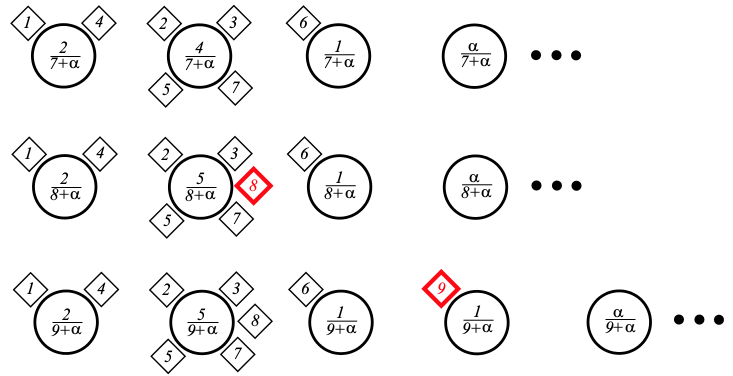
\includegraphics[width=1\textwidth]{np/dp/crp}
	\caption{(Figure from Suddherth PhD) Chinese restaurant process interpretation of the partitions induced by the Dirichlet process $\DP(\alpha, H)$. Tables (circles) are analogous to clusters, and customers (diamonds) to a series of observations. \emph{Top row}: A starting configuration, in which seven customers occupy three tables. Each table is labeled with the probability that the next customer sits there. \emph{Middle row}: New customers sit at occupied table $k$ with probability proportional to the number of previously seated diners $N_k$. In this example, the eighth customer joins the most popular, and hence likely, table. \emph{Bottom row}: Customers may also sit at one of the infinitely many unoccupied tables. The ninth diner does this.}
\end{figure}

The number of occupied tables $K$ almost surely approaches $\alpha \log(N)$ as $N \to \infty$.
\subsection{Dirichlet process mixtures}
The purpose is to cluster observations. We can't model continuous observations directly using a Dirichlet processes because the samples from them are almost surely discrete probability measures. Also, the posterior measure assigned to $x_i$ would never beinfluenced by observations $x_j \neq x_i$, regardless of their proximity.

The Dirichlet process mixtures model is as follows:
\begin{align*}
	G 				&\sim \DP(\alpha, H) \\
	\bar \theta_n	&\sim G 				& n = 1, \dotsc, N \\
	x_n				&\sim F(\bar \theta_n)
\end{align*}
where $G$ is being sampled from $\DP(\alpha, H)$ via the stick-breaking construction:
\begin{align*}
	\vec \pi 	&\sim \GEM(\alpha)	& \vec \pi = (\pi_1, \pi_2, \dotsc)\\
	\theta_k	&\sim H(\lambda)	& k = 1, 2, \dotsc \\
	G(\theta)	&= \sum_{k = 1}^\infty \pi_k \delta(\theta, \theta_k)
\end{align*}
this solves the problem of inability of the $\DP$ to model the distribution of observations directly. Now two observations $x_i, x_j$ are considered to be from the same cluster of $\bar \theta_n$ if both are $\sim F(\bar \theta_n)$.
\chapter{Probabilistic programming}
\section{Testing}
\subsection{Unit and measure tests}
Calculate KL divergences for discrete sample spaces and KS test statistics for continuous sample spaces.
\subsection{Conditional measure tests}
\subsubsection{ERPs}
The purpose is to test whether the \verb!*-lnpdf! functions work. For some distributions $f$ and $g$, if we \verb!assume! $\vec\theta \sim f$, then \verb!observe! $\mathcal D = \{y_n : y_n \sim g(\dotsc, \vec \theta)\}$, and finally \verb!predict! $\vec\theta \mid \mathcal D$, the inference engine will evaluate the \verb!*-lnpdf! functions of $g$ in order to characterise $\tilde p(\vec x \mid \vec y) \propto \tilde p(\vec y, \vec x) = \prod_n p(y_n \mid \theta_{t_n}, \vec x_n) \tilde p(\vec x_n \mid \vec x_{n - 1})$. We can then test whether the \verb!predict!'s follow the true distribution of $\vec\theta \mid \mathcal D$. Using this fact and taking advantage of conjugate pairs described in Chapter~\ref{chapter:par-est} and on Wikipedia, we can test the ERPs in the system as follows.

\begin{table}[h]
\begin{tabular}{ll}
\toprule
Bernoulli & \\
\midrule
$\theta \sim \Beta(\alpha, \beta)$								& \texttt{[assume theta (beta a b)]} \\
$x \mid \theta \sim \Ber(\theta)$								& \texttt{[observe (flip theta) x1] $\cdots$} \\
$\mathcal D = \{x_n\}$											& \texttt{[observe (flip theta) xN]} \\
$\theta \mid \mathcal D \sim \Beta(\alpha + N_1, \beta + N_0)$	& \texttt{[predict theta]} \\
\bottomrule
\end{tabular}
\end{table}

\begin{table}[h]
\begin{tabular}{ll}
\toprule
Binomial & \\
\midrule
$\theta \sim \Beta(\alpha, \beta)$													& \texttt{[assume theta (beta a b)]} \\
$x \mid \theta \sim \Bin(T, \theta)$												& \texttt{[observe (binomial theta T) x1] $\cdots$} \\
$\mathcal D = \{x_n\}$																& \texttt{[observe (binomial theta T) xN]} \\
$\theta \mid \mathcal D \sim \Beta(\alpha + \sum_n x_n, \beta + TN - \sum_n x_n)$	& \texttt{[predict theta]} \\
\bottomrule
\end{tabular}
\end{table}

\begin{table}[h]
\begin{tabular}{ll}
\toprule
Poisson & \\
\midrule
$\lambda \sim \Gammadist(\alpha, \beta)$											& \texttt{[assume l (gamma a b)]} \\
$x \mid \theta \sim \Poi(\lambda)$													& \texttt{[observe (poisson l) x1] $\cdots$} \\
$\mathcal D = \{x_n\}$																& \texttt{[observe (poisson l) xN]} \\
$\lambda \mid \mathcal D \sim \Gammadist(\alpha + \sum_n x_n, \beta + N)$			& \texttt{[predict l]} \\
\bottomrule
\end{tabular}
\end{table}

\begin{table}[h]
\begin{tabular}{ll}
\toprule
Categorical & \\
\midrule
$\vec\theta \sim \Dir(\vec\alpha), \vec\theta,\vec\alpha \in \mathbb R^K$			& \texttt{[assume ...]} \\
$x \mid \vec\theta \sim \Dir(\vec\theta)$											& \texttt{[observe ...] $\cdots$} \\
$\mathcal D = \{x_n\}$																& \texttt{[observe ...]} \\
$\vec\theta \mid \mathcal D \sim \Dir(\vec\alpha + (n_1, \dotsc, n_K)^T)$			& \texttt{[predict ...]} \\
\bottomrule
\end{tabular}
\end{table}

\begin{table}[h]
\begin{tabular}{ll}
\toprule
Univariate Normal with known variance & \\
\midrule
Fix $\sigma^2$																		& \texttt{[assume var \#var\#]} \\
$\mu \sim \Gauss(\mu_0, \sigma_0^2)$												& \texttt{[assume mu (normal mu0 var0)]} \\
$x \mid \vec\theta \sim \Gauss(\mu, \sigma^2)$										& \texttt{[observe (normal mu var) x1] $\cdots$} \\
$\mathcal D = \{x_n\}$																& \texttt{[observe (normal mu var) xN]} \\
$\mu \mid \mathcal D \sim \Gauss\left(\frac{\frac{\mu_0}{\sigma_0^2} + \frac{\sum_n x_n}{\sigma^2}}{\frac{1}{\sigma_0^2} + \frac{N}{\sigma^2}}, \left(\frac{1}{\sigma_0^2} + \frac{N}{\sigma^2}\right)^{-1}\right)$		& \texttt{[predict mu]} \\
\bottomrule
\end{tabular}
\end{table}

% \begin{table}[h]
% \begin{tabular}{ll}
% \toprule
% Uniform & \\
% \midrule
% $\theta \sim \Pareto(\mu_0, \sigma_0^2)$												& \texttt{[assume mu (normal mu0 var0)]} \\
% $x \mid \vec\theta \sim \Gauss(\mu, \sigma^2)$										& \texttt{[assume x (normal mu var)]} \\
% $\mathcal D = \{x_n\}$																& \texttt{[observe x x1]} $\cdots$ \texttt{[observe x xN]} \\
% $\mu \mid \mathcal D \sim \Gauss\left(\frac{\frac{\mu_0}{\sigma_0^2} + \frac{\sum_n x_n}{\sigma^2}}{\frac{1}{\sigma_0^2} + \frac{N}{\sigma^2}}, \left(\frac{1}{\sigma_0^2} + \frac{N}{\sigma^2}\right)^{-1}\right)$		& \texttt{[predict mu]} \\
% \bottomrule
% \end{tabular}
% \end{table}
\chapter{Weekly meetings for 4yp}
\section{MT14 -- Week 1}
\begin{itemize}
	\item Implement measure and conditional measure tests to test the ERPs.
	\item Research continuous integration (Jenkins, etc.)
	\item Study Dirichlet processes
	\item Research stuff
		\begin{itemize}
			\item Improve RDB by sampling from ?? half of the time instead of sampling from the prior.
			\item Sample ERPs (?) in a discretised manner in order to cover more of the sample space.
		\end{itemize}
\end{itemize}

\appendix
\chapter{Particle filter animation}
Needs to be opened in Adobe Reader.
\animategraphics[controls, width=1\linewidth]{0.3}{animations/particle-filter/}{1}{36}

\bibliography{bibliography}

\end{document}